\chapter{Results}
\label{sec:results}


\section{Presentation of Collected Data}
\subsection{Overview of Interviews}
We conducted semi-structured interviews with 16 native Swedish speakers (10 M/6F, age 23-78), each lasting 1-3 minutes. Each participant was interviewed for two different scenarios, resulting in 32 different recordings. All interviews were audio-recorded in a quiet room and elicited two target emotions – anger and happiness – via open-ended prompts (e.g. “Is there anything in society that makes you upset? What? How does that make you feel?”; “Can you remember one time you felt really proud of yourself?”). The participants rated their perceived emotions on a 1-6 scale immediately after each scenario. The rated emotions covered the basic 5 emotions mentioned in this report: anger, joy, sadness, fear, and surprise. 

Table~\ref{tab:interview_table} presents the participants ID, gender, age, and self-assessed scores for their perceived emotions for respective interview scenario.
\begin{table}[H]
    \centering
    \begin{tabular}{|lrl|
    >{\columncolor[HTML]{FBE2D5}}l 
    >{\columncolor[HTML]{FBE2D5}}l 
    >{\columncolor[HTML]{FBE2D5}}l 
    >{\columncolor[HTML]{FBE2D5}}l 
    >{\columncolor[HTML]{FBE2D5}}l |
    >{\columncolor[HTML]{DAF2D0}}l 
    >{\columncolor[HTML]{DAF2D0}}l 
    >{\columncolor[HTML]{DAF2D0}}l 
    >{\columncolor[HTML]{DAF2D0}}l 
    >{\columncolor[HTML]{DAF2D0}}l |}
    \hline
    \multicolumn{3}{|c|}{Participant}                                                                                                 & \multicolumn{5}{c|}{\cellcolor[HTML]{F7C7AC}Negative}                                                                                                                                                     & \multicolumn{5}{c|}{\cellcolor[HTML]{B5E6A2}Positive}                                                                                                                                                                                                  \\ \hline
    \multicolumn{1}{|l|}{\cellcolor[HTML]{D9D9D9}ID} & \multicolumn{1}{l|}{\cellcolor[HTML]{D9D9D9}M/F} & \cellcolor[HTML]{D9D9D9}Age & \multicolumn{1}{l|}{\cellcolor[HTML]{FBE2D5}A} & \multicolumn{1}{l|}{\cellcolor[HTML]{FBE2D5}J} & \multicolumn{1}{l|}{\cellcolor[HTML]{FBE2D5}Sad} & \multicolumn{1}{l|}{\cellcolor[HTML]{FBE2D5}F} & Sur & \multicolumn{1}{c|}{\cellcolor[HTML]{DAF2D0}A} & \multicolumn{1}{c|}{\cellcolor[HTML]{DAF2D0}J} & \multicolumn{1}{c|}{\cellcolor[HTML]{DAF2D0}Sad} & \multicolumn{1}{c|}{\cellcolor[HTML]{DAF2D0}F} & \multicolumn{1}{c|}{\cellcolor[HTML]{DAF2D0}Sur} \\ \hline
    \multicolumn{1}{|l|}{1}                          & \multicolumn{1}{r|}{M}                           & 23                          & \multicolumn{1}{l|}{\cellcolor[HTML]{FBE2D5}5} & \multicolumn{1}{l|}{\cellcolor[HTML]{FBE2D5}1} & \multicolumn{1}{l|}{\cellcolor[HTML]{FBE2D5}3}   & \multicolumn{1}{l|}{\cellcolor[HTML]{FBE2D5}1} & 1   & \multicolumn{1}{l|}{\cellcolor[HTML]{DAF2D0}1} & \multicolumn{1}{l|}{\cellcolor[HTML]{DAF2D0}6} & \multicolumn{1}{l|}{\cellcolor[HTML]{DAF2D0}1}   & \multicolumn{1}{l|}{\cellcolor[HTML]{DAF2D0}1} & 4                                                \\ \hline
    \multicolumn{1}{|l|}{2}                          & \multicolumn{1}{r|}{M}                           & 26                          & \multicolumn{1}{l|}{\cellcolor[HTML]{FBE2D5}6} & \multicolumn{1}{l|}{\cellcolor[HTML]{FBE2D5}1} & \multicolumn{1}{l|}{\cellcolor[HTML]{FBE2D5}3}   & \multicolumn{1}{l|}{\cellcolor[HTML]{FBE2D5}4} & 1   & \multicolumn{1}{l|}{\cellcolor[HTML]{DAF2D0}1} & \multicolumn{1}{l|}{\cellcolor[HTML]{DAF2D0}6} & \multicolumn{1}{l|}{\cellcolor[HTML]{DAF2D0}1}   & \multicolumn{1}{l|}{\cellcolor[HTML]{DAF2D0}2} & 1                                                \\ \hline
    \multicolumn{1}{|l|}{3}                          & \multicolumn{1}{r|}{F}                           & 27                          & \multicolumn{1}{l|}{\cellcolor[HTML]{FBE2D5}4} & \multicolumn{1}{l|}{\cellcolor[HTML]{FBE2D5}1} & \multicolumn{1}{l|}{\cellcolor[HTML]{FBE2D5}6}   & \multicolumn{1}{l|}{\cellcolor[HTML]{FBE2D5}1} & 2   & \multicolumn{1}{l|}{\cellcolor[HTML]{DAF2D0}1} & \multicolumn{1}{l|}{\cellcolor[HTML]{DAF2D0}6} & \multicolumn{1}{l|}{\cellcolor[HTML]{DAF2D0}1}   & \multicolumn{1}{l|}{\cellcolor[HTML]{DAF2D0}1} & 3                                                \\ \hline
    \multicolumn{1}{|l|}{4}                          & \multicolumn{1}{r|}{M}                           & 29                          & \multicolumn{1}{l|}{\cellcolor[HTML]{FBE2D5}2} & \multicolumn{1}{l|}{\cellcolor[HTML]{FBE2D5}1} & \multicolumn{1}{l|}{\cellcolor[HTML]{FBE2D5}3}   & \multicolumn{1}{l|}{\cellcolor[HTML]{FBE2D5}2} & 1   & \multicolumn{1}{l|}{\cellcolor[HTML]{DAF2D0}1} & \multicolumn{1}{l|}{\cellcolor[HTML]{DAF2D0}4} & \multicolumn{1}{l|}{\cellcolor[HTML]{DAF2D0}2}   & \multicolumn{1}{l|}{\cellcolor[HTML]{DAF2D0}2} & 2                                                \\ \hline
    \multicolumn{1}{|l|}{5}                          & \multicolumn{1}{r|}{F}                           & 28                          & \multicolumn{1}{l|}{\cellcolor[HTML]{FBE2D5}4} & \multicolumn{1}{l|}{\cellcolor[HTML]{FBE2D5}1} & \multicolumn{1}{l|}{\cellcolor[HTML]{FBE2D5}4}   & \multicolumn{1}{l|}{\cellcolor[HTML]{FBE2D5}1} & 2   & \multicolumn{1}{l|}{\cellcolor[HTML]{DAF2D0}1} & \multicolumn{1}{l|}{\cellcolor[HTML]{DAF2D0}5} & \multicolumn{1}{l|}{\cellcolor[HTML]{DAF2D0}1}   & \multicolumn{1}{l|}{\cellcolor[HTML]{DAF2D0}1} & 5                                                \\ \hline
    \multicolumn{1}{|l|}{6}                          & \multicolumn{1}{r|}{M}                           & 25                          & \multicolumn{1}{l|}{\cellcolor[HTML]{FBE2D5}2} & \multicolumn{1}{l|}{\cellcolor[HTML]{FBE2D5}2} & \multicolumn{1}{l|}{\cellcolor[HTML]{FBE2D5}1}   & \multicolumn{1}{l|}{\cellcolor[HTML]{FBE2D5}1} & 1   & \multicolumn{1}{l|}{\cellcolor[HTML]{DAF2D0}1} & \multicolumn{1}{l|}{\cellcolor[HTML]{DAF2D0}3} & \multicolumn{1}{l|}{\cellcolor[HTML]{DAF2D0}1}   & \multicolumn{1}{l|}{\cellcolor[HTML]{DAF2D0}1} & 1                                                \\ \hline
    \multicolumn{1}{|l|}{8}                          & \multicolumn{1}{r|}{M}                           & 27                          & \multicolumn{1}{l|}{\cellcolor[HTML]{FBE2D5}3} & \multicolumn{1}{l|}{\cellcolor[HTML]{FBE2D5}1} & \multicolumn{1}{l|}{\cellcolor[HTML]{FBE2D5}2}   & \multicolumn{1}{l|}{\cellcolor[HTML]{FBE2D5}1} & 2   & \multicolumn{1}{l|}{\cellcolor[HTML]{DAF2D0}1} & \multicolumn{1}{l|}{\cellcolor[HTML]{DAF2D0}5} & \multicolumn{1}{l|}{\cellcolor[HTML]{DAF2D0}1}   & \multicolumn{1}{l|}{\cellcolor[HTML]{DAF2D0}1} & 1                                                \\ \hline
    \multicolumn{1}{|l|}{9}                          & \multicolumn{1}{r|}{F}                           & 26                          & \multicolumn{1}{l|}{\cellcolor[HTML]{FBE2D5}3} & \multicolumn{1}{l|}{\cellcolor[HTML]{FBE2D5}1} & \multicolumn{1}{l|}{\cellcolor[HTML]{FBE2D5}3}   & \multicolumn{1}{l|}{\cellcolor[HTML]{FBE2D5}1} & 1   & \multicolumn{1}{l|}{\cellcolor[HTML]{DAF2D0}1} & \multicolumn{1}{l|}{\cellcolor[HTML]{DAF2D0}5} & \multicolumn{1}{l|}{\cellcolor[HTML]{DAF2D0}1}   & \multicolumn{1}{l|}{\cellcolor[HTML]{DAF2D0}1} & 1                                                \\ \hline
    \multicolumn{1}{|l|}{10}                         & \multicolumn{1}{r|}{F}                           & 78                          & \multicolumn{1}{l|}{\cellcolor[HTML]{FBE2D5}5} & \multicolumn{1}{l|}{\cellcolor[HTML]{FBE2D5}1} & \multicolumn{1}{l|}{\cellcolor[HTML]{FBE2D5}3}   & \multicolumn{1}{l|}{\cellcolor[HTML]{FBE2D5}2} & 4   & \multicolumn{1}{l|}{\cellcolor[HTML]{DAF2D0}1} & \multicolumn{1}{l|}{\cellcolor[HTML]{DAF2D0}6} & \multicolumn{1}{l|}{\cellcolor[HTML]{DAF2D0}4}   & \multicolumn{1}{l|}{\cellcolor[HTML]{DAF2D0}1} & 1                                                \\ \hline
    \multicolumn{1}{|l|}{11}                         & \multicolumn{1}{r|}{F}                           & 27                          & \multicolumn{1}{l|}{\cellcolor[HTML]{FBE2D5}3} & \multicolumn{1}{l|}{\cellcolor[HTML]{FBE2D5}3} & \multicolumn{1}{l|}{\cellcolor[HTML]{FBE2D5}2}   & \multicolumn{1}{l|}{\cellcolor[HTML]{FBE2D5}1} & 1   & \multicolumn{1}{l|}{\cellcolor[HTML]{DAF2D0}1} & \multicolumn{1}{l|}{\cellcolor[HTML]{DAF2D0}6} & \multicolumn{1}{l|}{\cellcolor[HTML]{DAF2D0}1}   & \multicolumn{1}{l|}{\cellcolor[HTML]{DAF2D0}1} & 1                                                \\ \hline
    \multicolumn{1}{|l|}{12}                         & \multicolumn{1}{r|}{M}                           & 58                          & \multicolumn{1}{l|}{\cellcolor[HTML]{FBE2D5}1} & \multicolumn{1}{l|}{\cellcolor[HTML]{FBE2D5}3} & \multicolumn{1}{l|}{\cellcolor[HTML]{FBE2D5}1}   & \multicolumn{1}{l|}{\cellcolor[HTML]{FBE2D5}2} & 1   & \multicolumn{1}{l|}{\cellcolor[HTML]{DAF2D0}1} & \multicolumn{1}{l|}{\cellcolor[HTML]{DAF2D0}6} & \multicolumn{1}{l|}{\cellcolor[HTML]{DAF2D0}1}   & \multicolumn{1}{l|}{\cellcolor[HTML]{DAF2D0}1} & 3                                                \\ \hline
    \multicolumn{1}{|l|}{13}                         & \multicolumn{1}{r|}{F}                           & 54                          & \multicolumn{1}{l|}{\cellcolor[HTML]{FBE2D5}4} & \multicolumn{1}{l|}{\cellcolor[HTML]{FBE2D5}1} & \multicolumn{1}{l|}{\cellcolor[HTML]{FBE2D5}4}   & \multicolumn{1}{l|}{\cellcolor[HTML]{FBE2D5}3} & 1   & \multicolumn{1}{l|}{\cellcolor[HTML]{DAF2D0}1} & \multicolumn{1}{l|}{\cellcolor[HTML]{DAF2D0}6} & \multicolumn{1}{l|}{\cellcolor[HTML]{DAF2D0}1}   & \multicolumn{1}{l|}{\cellcolor[HTML]{DAF2D0}1} & 1                                                \\ \hline
    \multicolumn{1}{|l|}{14}                         & \multicolumn{1}{r|}{M}                           & 20                          & \multicolumn{1}{l|}{\cellcolor[HTML]{FBE2D5}1} & \multicolumn{1}{l|}{\cellcolor[HTML]{FBE2D5}3} & \multicolumn{1}{l|}{\cellcolor[HTML]{FBE2D5}1}   & \multicolumn{1}{l|}{\cellcolor[HTML]{FBE2D5}2} & 2   & \multicolumn{1}{l|}{\cellcolor[HTML]{DAF2D0}1} & \multicolumn{1}{l|}{\cellcolor[HTML]{DAF2D0}4} & \multicolumn{1}{l|}{\cellcolor[HTML]{DAF2D0}1}   & \multicolumn{1}{l|}{\cellcolor[HTML]{DAF2D0}1} & 3                                                \\ \hline
    \multicolumn{1}{|l|}{15}                         & \multicolumn{1}{r|}{M}                           & 30                          & \multicolumn{1}{l|}{\cellcolor[HTML]{FBE2D5}3} & \multicolumn{1}{l|}{\cellcolor[HTML]{FBE2D5}2} & \multicolumn{1}{l|}{\cellcolor[HTML]{FBE2D5}2}   & \multicolumn{1}{l|}{\cellcolor[HTML]{FBE2D5}3} & 1   & \multicolumn{1}{l|}{\cellcolor[HTML]{DAF2D0}2} & \multicolumn{1}{l|}{\cellcolor[HTML]{DAF2D0}5} & \multicolumn{1}{l|}{\cellcolor[HTML]{DAF2D0}1}   & \multicolumn{1}{l|}{\cellcolor[HTML]{DAF2D0}1} & 1                                                \\ \hline
    \multicolumn{1}{|l|}{16}                         & \multicolumn{1}{r|}{M}                           & 25                          & \multicolumn{1}{l|}{\cellcolor[HTML]{FBE2D5}4} & \multicolumn{1}{l|}{\cellcolor[HTML]{FBE2D5}1} & \multicolumn{1}{l|}{\cellcolor[HTML]{FBE2D5}2}   & \multicolumn{1}{l|}{\cellcolor[HTML]{FBE2D5}1} & 1   & \multicolumn{1}{l|}{\cellcolor[HTML]{DAF2D0}1} & \multicolumn{1}{l|}{\cellcolor[HTML]{DAF2D0}6} & \multicolumn{1}{l|}{\cellcolor[HTML]{DAF2D0}1}   & \multicolumn{1}{l|}{\cellcolor[HTML]{DAF2D0}1} & 1                                                \\ \hline
    \end{tabular}
    \caption{Participant table. A: Anger, J: Joy, Sad: Sadness, F: Fear, Sur: Surprise.}
    \label{tab:interview_table}
\end{table}

\subsection{Data Collection for RQ1: Vocal Features \& Speech}
The collected audio recordings from the 32 interviews were processed for research questions 1 to specifically focus on vocal features and speech-based emotion recognition. 
\subsubsection{Vocal Feature Extraction (Praat Parselmouth)}
Audio recordings were processed with Praat Parselmouth. Vocal parameters were extracted from each recording, which have been validatied by Swedish emotion research on vocal markers \autocite{Ekberg2023}. 
\begin{itemize}
    \item Pitch: mean pitch in Hz and semitones (ST). 
    \item Intensity: mean intensity measured in decibels (dB). 
    \item Voice Quality Metrics: Harmonic-to-Noise Ratio (HNR), jitter (local frequency perturbation), shimmer (local ampliture perturbation). 
\end{itemize}
These acoustic features were then categorized into discrete emotional labels (anger, joy, sadness, fear, surprise) based on thresholds and criteria defined in prior Swedish research \autocite{Ekberg2023}. 

\subsubsection{Speech-Based Emotion Recognition (Hume AI)}
The same audio were analyzed with Hume AI, that provided probability distributions across several emotions, where the five targeted emotions was filtered from. 
The results were normalized according to ADD THAT PART INTO METHOD FROM PDF REFER TO HERE. 

\subsubsection{Data Structure}
The extracted vocal features, custom emotion categorizations of vocal features, and Hume AI outputs were combined for each recording and stored in JSON format, to enable direct comparison and further analysis. All data is normalized to sum up to 1 before loaded into the JSON files. 
Table \ref{tab:summary_vocal_features_by_sentiment} includes the mean values and standard diversion for the analysed features (pitch, intensity, HNR, jitter, shimmer) seperated by sentiment. 
Filtered Hume probabilities are presented in Table \ref{tab:summary_hume_by_sentiment} as mean values with standardized diversion for positive and negative recordings.

The custom categorization of emotion based on vocal features are presented as mean values including standard diversions for positive and negative sentiments in Table~\ref{tab:summary_praat_by_sentiment}. 

  \begin{table}[H]
    \centering
    \begin{subtable}{0.45\textwidth}
      \centering
      \caption*{\textbf{Negative Clips}}
      \begin{tabular}{lrr}
        \toprule
        \textbf{Feature}         & \textbf{Mean}    & \textbf{Std}    \\
        \midrule
        mean\_pitch\_st          & –0,1606          & 5,9616          \\
        mean\_pitch\_hz          & 157,1044         & 53,2213         \\
        mean\_intensity\_db      & 62,9767          & 2,3435          \\
        mean\_hnr\_db            & 5,7883           & 5,8332          \\
        jitter\_local            & 0,0246           & 0,0032          \\
        shimmer\_local           & 0,1219           & 0,0267          \\
        \bottomrule
      \end{tabular}
    \end{subtable}\hfill
    \begin{subtable}{0.45\textwidth}
      \centering
      \caption*{\textbf{Positive Clips}}
      \begin{tabular}{lrr}
        \toprule
        \textbf{Feature}         & \textbf{Mean}    & \textbf{Std}    \\
        \midrule
        mean\_pitch\_st          & –0,6688          & 6,0049          \\
        mean\_pitch\_hz          & 152,8906         & 54,6353         \\
        mean\_intensity\_db      & 63,7063          & 3,0511          \\
        mean\_hnr\_db            & 5,3269           & 5,8034          \\
        jitter\_local            & 0,0253           & 0,0046          \\
        shimmer\_local           & 0,1286           & 0,0218          \\
        \bottomrule
      \end{tabular}
    \end{subtable}
    \caption{Summary Statistics: Vocal Features by Sentiment}
    \label{tab:summary_vocal_features_by_sentiment}
  \end{table}
  
  
  \begin{table}[H]
    \centering
    \begin{subtable}{0.45\textwidth}
      \centering
      \caption*{\textbf{Positive Clips}}
      \begin{tabular}{lrr}
        \toprule
        \textbf{Metric}      & \textbf{Mean}  & \textbf{Std}   \\
        \midrule
        hume\_anger          & 0,2262         & 0,0584         \\
        hume\_fear           & 0,1485         & 0,0513         \\
        hume\_joy            & 0,3318         & 0,1279         \\
        hume\_sadness        & 0,1673         & 0,0644         \\
        hume\_surprise       & 0,1264         & 0,0209         \\
        \bottomrule
      \end{tabular}
    \end{subtable}\hfill
    \begin{subtable}{0.45\textwidth}
      \centering
      \caption*{\textbf{Negative Clips}}
      \begin{tabular}{lrr}
        \toprule
        \textbf{Metric}      & \textbf{Mean}  & \textbf{Std}   \\
        \midrule
        hume\_anger          & 0,2832         & 0,0751         \\
        hume\_fear           & 0,1523         & 0,0372         \\
        hume\_joy            & 0,2758         & 0,0951         \\
        hume\_sadness        & 0,1771         & 0,0691         \\
        hume\_surprise       & 0,1117         & 0,0205         \\
        \bottomrule
      \end{tabular}
    \end{subtable}
    \caption{Summary Statistics: Hume AI Probabilities by Sentiment}
    \label{tab:summary_hume_by_sentiment}
  \end{table}
  

  \begin{table}[H]
    \centering
    \begin{subtable}{0.45\textwidth}
      \centering
      \caption*{\textbf{Positive Clips}}
      \begin{tabular}{lrr}
        \toprule
        \textbf{Metric}      & \textbf{Mean}  & \textbf{Std}   \\
        \midrule
        custom\_anger        & 0,2066         & 0,0031         \\
        custom\_joy          & 0,2036         & 0,0039         \\
        custom\_fear         & 0,2028         & 0,0079         \\
        custom\_sadness      & 0,1913         & 0,0027         \\
        custom\_surprise     & 0,1956         & 0,0062         \\
        \bottomrule
      \end{tabular}
    \end{subtable}\hfill
    \begin{subtable}{0.45\textwidth}
      \centering
      \caption*{\textbf{Negative Clips}}
      \begin{tabular}{lrr}
        \toprule
        \textbf{Metric}      & \textbf{Mean}  & \textbf{Std}   \\
        \midrule
        custom\_anger        & 0,2064         & 0,0034         \\
        custom\_joy          & 0,2043         & 0,0041         \\
        custom\_fear         & 0,2042         & 0,0087         \\
        custom\_sadness      & 0,1906         & 0,0032         \\
        custom\_surprise     & 0,1946         & 0,0063         \\
        \bottomrule
      \end{tabular}
    \end{subtable}
    \caption{Summary Statistics: Custom Emotion Categorization Scores by Sentiment}
    \label{tab:summary_praat_by_sentiment}
  \end{table}
  
  
  

\subsubsection{Segment-Level Data}
Certain analyses in RQ1 rely on time-segmented data. For each recording, Hume AI returns emotion probabilities at regular time segments, an example of this is presented in Table~\ref{tab:segments_hume_example}. 
In the data analysis, we extract the same set of acoustic features from matching time intervals with Praat, enabling time-to-time comparisons across modalities.
\begin{table}[H]
    \centering
    
    \begin{tabular}{rrrrrrl}
      \toprule
      \textbf{time (s)} & \textbf{anger} & \textbf{fear} & \textbf{joy} & \textbf{sadness} & \textbf{surprise} \\
      \midrule
      1,47    & 0,2332  & 0,1590 & 0,4244 & 0,1214 & 0,0620 \\
      5,15    & 0,1469  & 0,0342 & 0,6693 & 0,0110 & 0,1387 \\
      8,27    & 0,0993  & 0,0259 & 0,7804 & 0,0184 & 0,0759 \\
      \dots   & \dots   & \dots  & \dots  & \dots  & \dots  \\
      43,2342 & 0,1216  & 0,0837 & 0,5861 & 0,0500 & 0,1586 \\
      \bottomrule
    \end{tabular}
    \caption{Segment‐Level Hume Probabilities for clip: id\_001\_neg}
    \label{tab:segments_hume_example}
  \end{table}
  

\subsection{Data Collection for RQ2 and RQ3: Text, Speech and Self-Assessment}
\label{sec:datacoll_rq2_rq3}


The data collection for RQ2 and RQ3 is based on the same audio recordings as for RQ1. 
Each recording was transcribed and analyzed with NLP Cloud (text-based), to extract emotion probabilities from the transcription. The same audio was analyzed using Hume AI for speech-based emotion detection, resulting in paired emotion probability scores alongside self-reported emotion ratings. All scores were normalized for comparison.

The data was structured in JSON format, each audio object consists of five emotion labels from each data type (Hume, NLP, Self). 


Table~\ref{tab:rq3_emotion-stats-combined} summarize the average emotion scores and standard deviations for both speech-based (Hume AI) and text-based (NLP Cloud) 
models across all clips in the dataset. 

\begin{table}[H]
    \centering
    \caption*{\textbf{All Recordings}}
    \begin{tabular}{lrrrrrr}
      \toprule
      \textbf{Emotion} & \textbf{Self Mean} & \textbf{Hume Mean} & \textbf{NLP Mean} & \textbf{Self Std} & \textbf{Hume Std} & \textbf{NLP Std} \\
      \midrule
      Anger    & 0,210 & 0,260 & 0,200 & 0,124 & 0,072 & 0,223 \\
      Joy      & 0,312 & 0,302 & 0,396 & 0,200 & 0,117 & 0,351 \\
      Sadness  & 0,190 & 0,167 & 0,181 & 0,105 & 0,065 & 0,138 \\
      Fear     & 0,136 & 0,150 & 0,093 & 0,061 & 0,045 & 0,092 \\
      Surprise & 0,149 & 0,118 & 0,129 & 0,082 & 0,022 & 0,089 \\
      \bottomrule
    \end{tabular}
    \caption{Means and standard deviations of self-reported, Hume, and NLP emotion intensities.}
    \label{tab:rq3_emotion-stats-combined}
  \end{table}
  
  The interviews were conducted with either a positive or negative orientation. Each recording was analyzed individually, and
  the data structure distinguishes between negative and positive audio files. The corresponding emotion scores from Hume AI and 
  NLP Cloud are presented in Table~\ref{tab:rq3_emotion-stats-pos} for positively oriented interviews, and in Table~\ref{tab:rq3_emotion-stats_neg}
  for negatively oriented interviews. Each table displays the mean and the standard deviation for the respective AI model's emotion probability. 
  \begin{table}[H]
    \centering
    \caption*{\textbf{Positive Recordings}}
    \begin{tabular}{lrrrrrr}
      \toprule
      \textbf{Emotion} & \textbf{Self Mean} & \textbf{Hume Mean} & \textbf{NLP Mean} & \textbf{Self Std} & \textbf{Hume Std} & \textbf{NLP Std} \\
      \midrule
      Anger    & 0,103 & 0,227 & 0,015 & 0,032 & 0,060 & 0,057 \\
      Joy      & 0,497 & 0,333 & 0,708 & 0,081 & 0,132 & 0,169 \\
      Sadness  & 0,117 & 0,163 & 0,067 & 0,059 & 0,065 & 0,062 \\
      Fear     & 0,108 & 0,148 & 0,040 & 0,033 & 0,052 & 0,067 \\
      Surprise & 0,173 & 0,126 & 0,171 & 0,098 & 0,022 & 0,096 \\
      \bottomrule
    \end{tabular}
    \caption{Means and standard deviations of self-reported, Hume, and NLP emotion intensities for positive recordings.}
    \label{tab:rq3_emotion-stats-pos}
  \end{table}

\begin{table}[H]
    \centering
    \caption*{\textbf{Negative Recordings}}
    \begin{tabular}{lrrrrrr}
      \toprule
      \textbf{Emotion} & \textbf{Self Mean} & \textbf{Hume Mean} & \textbf{NLP Mean} & \textbf{Self Std} & \textbf{Hume Std} & \textbf{NLP Std} \\
      \midrule
      Anger    & 0,305 & 0,289 & 0,363 & 0,092 & 0,072 & 0,183 \\
      Joy      & 0,148 & 0,275 & 0,121 & 0,106 & 0,098 & 0,205 \\
      Sadness  & 0,254 & 0,171 & 0,282 & 0,095 & 0,066 & 0,103 \\
      Fear     & 0,161 & 0,152 & 0,141 & 0,069 & 0,038 & 0,087 \\
      Surprise & 0,128 & 0,112 & 0,092 & 0,059 & 0,021 & 0,064 \\
      \bottomrule
    \end{tabular}
    \caption{Means and standard deviations of self-reported, Hume, and NLP emotion intensities for negative recordings.}
    \label{tab:rq3_emotion-stats_neg}
  \end{table}


%%%%%%%%%%%%%%%%%%%%%%%%%%%%%%%%%%%%%%%%%%%%%%%%%%%%%%%%%%%%%%%%%%%%%%%%%%%%%%%%%%%%%
                        %%%%%%%%%%%%%%%%% RQ1 %%%%%%%%%%%%%%%%%
%%%%%%%%%%%%%%%%%%%%%%%%%%%%%%%%%%%%%%%%%%%%%%%%%%%%%%%%%%%%%%%%%%%%%%%%%%%%%%%%%%%%%       
\section{Data Analysis for RQ1: Vocal Features \& Speech Emotion Recognition}
The first research question explores how vocal features correlates with AI-based emotion detection in conversational Swedish speech. 
To analyse this, acoustic features such as pitch, intensity, jitter, shimmer and HNR were extracted using Praat Parselmouth and compared with emotion 
scores from the speech-based model Hume AI. A custom categorization method based on Swedish vocal emotion research \autocite{Ekberg2023} were tested for comparison. 
The goal with this analysis was to explore if these vocal markers could explain or predict how speech-based AI systems interpret emotional expressions in 
semi-structured, spontaneous speech in an interview setting. 

\subsection{Correlation Between Vocal Features and AI Emotion Scores (Hume AI)}
Figure \ref{fig:rq1-heatmaps} demonstrates heatmaps of the Pearson correlation coefficients between selected vocal features and Hume AI emotion labels across positive clips in Figure \ref{fig:hume_vocal_positive} and negative clips in Figure \ref{fig:hume_vocal_negative}. The results show generally weak correlations, with slightly stronger correlations for the negative recordings.  

\begin{figure}[!h]
    \centering 
    \begin{subfigure}[b]{0.45\textwidth}
        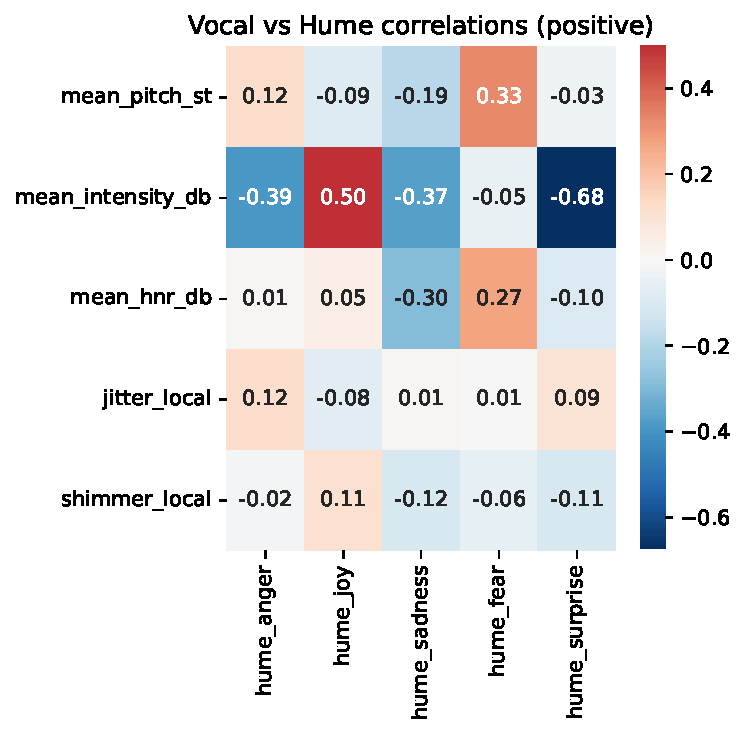
\includegraphics[width=\textwidth]{png/results/rq1_nr3/vocal_vs_hume_correlations_positive.png.pdf}
        \caption{Hume vs vocal features positive}
        \label{fig:hume_vocal_positive}
    \end{subfigure}
    \begin{subfigure}[b]{0.45\textwidth}
        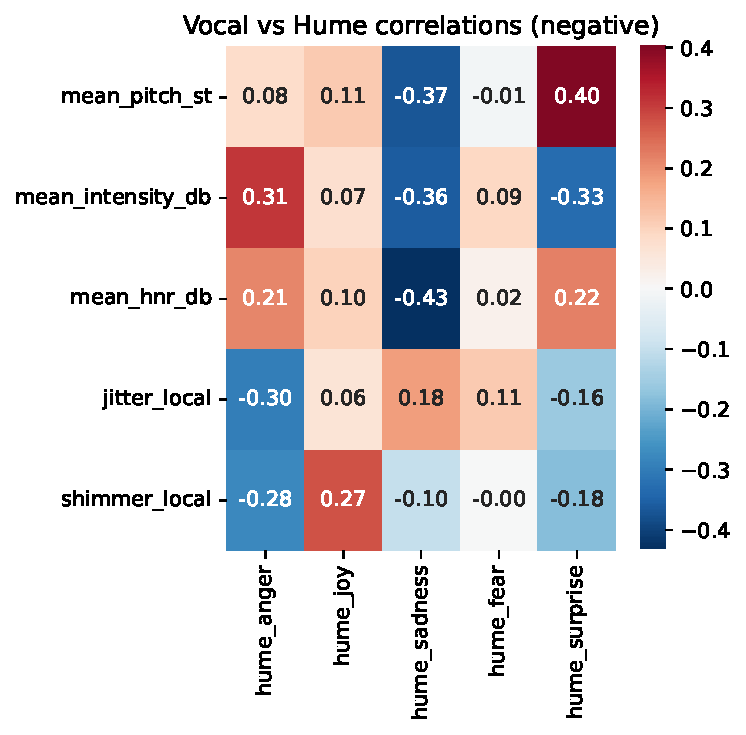
\includegraphics[width=\textwidth]{png/results/rq1_nr3/vocal_vs_hume_correlations_negative.png.pdf}
        \caption{Hume vs vocal features negative}        
        \label{fig:hume_vocal_negative}
    \end{subfigure}   
    \caption{Correlation Heatmaps between Hume AI and vocal features.}
    \label{fig:rq1-heatmaps}     
\end{figure}
Correlation values for positive interviews in Figure \ref{fig:hume_vocal_positive} ranging roughly between -0.7 and 0.5, most values suggest generally weaker correlations than the highest values. Stronger positive correlations 
suggests that certain feature is higher when Hume rates the correlating emotion. Negative correlations implies the opposite, low value of a certain feature for the correlated emotion. 
Mean intensity stands out from other vocal features with a moderate positive correlation with Hume Joy (r = 0.50), a moderate negative correlation with Hume Anger (r = -0.39), a moderate negative relationship with Hume sadness (r = -0.37) and a strong negative correlation with Hume Surprise (r = -0.68). 
Mean pitch shows strongest effect on Hume Fear (r = 0.30) and a moderate negative link with Hume Sadness (r = -0.21). 
Mean HNR has a moderate negative correlation with Hume Sadness (r = -0.30) as well it is moderately positively correlated with Hume Fear (r = 0.27). 
Jitter and shimmer remain near zero for most emotions in the positive clips, with none exceeding |r| = 0.13. This suggests that, in more positively oriented interviews, 
variation in pitch, intensity, and HNR capture the core emotion-related cues moderately, while jitter and shimmer have small predictive influence in semi-spontaneous speech during interview conversations. 

Figure \ref{fig:hume_vocal_negative} illustrates Pearson correlation values for negative clips in the dataset, again presenting generally weak effects even if slightly stronger correlations occur, approximately ranging between -0.5 and 0.5. 
The strongest relationship appears for sadness, where mean HNR shows a strong negative correlation (r = -0.43) and moderately negative correlated with pitch (r = -0.37) and intensity (r = -0.36). 
Anger had the highest positive correlation with intensity (r = 0.31) followed by a weak positive link with HNR (r = 0.21) and weak to moderate negative correlations with jitter (r = -0.30) and shimmer (r = -0.28). 
Correlations between vocal features and joy are all perceived weak, shimmer emerges as strongest (r = 0.27) compared to all other features (r < 0.11). 
Hume predicted fear presents coefficients indicating no linear correlation for all vocal features (r < 0.11). Surprise presents a moderate positive correlation with pitch (r = 0.36) and negative relationship with intensity (r = -0.33), other features are weakly correlated to the emotion.
Jitter and shimmer show similar relationships to Hume Fear (r ≈ 0.2). Shimmer has strongest correlation with Hume Anger, and a moderate relationship with Hume Joy. Jitter is moderately correlated with Anger as well and have a moderate correlation with Sadness where shimmer has almost no correlation. 

\medskip
Overall, the negative and positive diversion suggests that intensity consistently reflect Hume AI’s anger, sadness, and surprise predictions, and more prominent for joy in positive recordings and near zero for joy rated in negative contexts. 
Correlations between pitch and emotions predicted by Hume is generally weak and varying between the sentiment categories. 
 Jitter and shimmer remain minor indicators for positive conditions, while having moderate correlations with Hume anger and joy in negative recordings.

\subsection{Correlation with Praat-Based Emotion Scores}

\begin{figure}[H]
    \centering 
    \begin{subfigure}[b]{0.45\textwidth}
        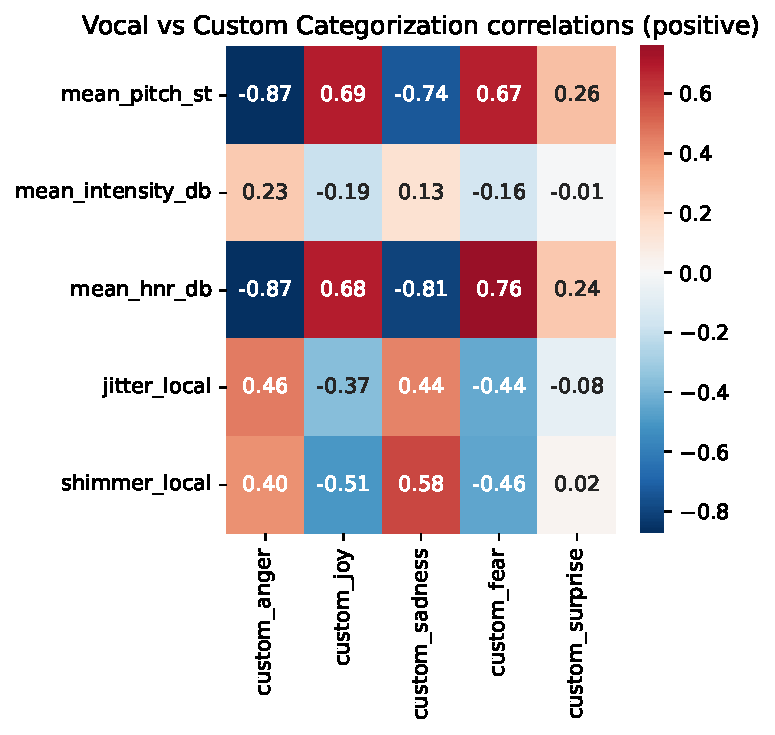
\includegraphics[width=\textwidth]{png/results/rq1_nr3/vocal_vs_custom_categorization_correlations_positive.png.pdf}
        \caption{Positive recordings.}
        \label{fig:custom_vocal_positive}
    \end{subfigure}
    \begin{subfigure}[b]{0.45\textwidth}
        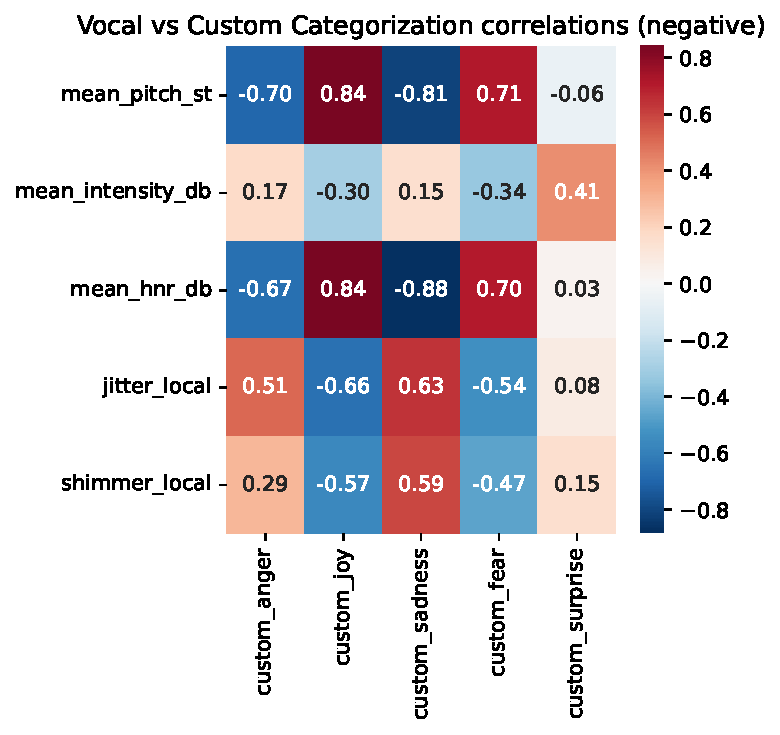
\includegraphics[width=\textwidth]{png/results/rq1_nr3/vocal_vs_custom_categorization_correlations_negative.png.pdf}
        \caption{Negative Recordings}        
        \label{fig:custom_vocal_negative}
    \end{subfigure} 
    \caption{Correlation heatmaps for custom categorized emotion scores vs. vocal features.}
    \label{fig:rq1_heatmaps_custom}       
\end{figure}
Figure~\ref{fig:rq1_heatmaps_custom} presents heatmaps of Pearson’s correlation r between selected vocal features and the emotion scores obtained from the custom emotion categorization 
function for Figure \ref{fig:custom_vocal_positive} positive oriented clips and Figure \ref{fig:custom_vocal_negative} negative clips. In contrast to the correlation results between Hume AI and vocal markers, these heatmaps present similar values and orientations for both negative and positive recordings, with values roughly ranging from -0.5 to 0.4. 
In positive recordings, pitch and HNR correlation coefficients shows a similar pattern where custom categorized sadness have the most distinct relationship (pitch r = 0.30, HNR r = 0.38). Pitch is weakly correlated with other custom categorized emotions, with a slightly hightened positive correlation with anger (r = 0.19) and negative with fear (r = -0.20).
HNR demonstrates the strongest correlations of all features, approaching a positive moderate relationship with anger (r = 0.28), while negatively correlated with fear (r = -0.32). 
Intensity shows a slight increase in correlation, yet below the threshold for moderate strength, for anger and sadness (r = 0.20). 
Jitter and shimmer have minor correlations with all custom categorized emotion labels (|r| < 0.13). 

Correlations for the negative subset have lower value distribution than the positive subset. Intensity and custom surprise present the singular strong negative correlation (r = -0.51). Subsequently, fear and intensity are moderately correlated (r = 0.33).
As for positive recordings, pitch and HNR demonstrate similar behaviors for all emotions - both have a similar weak positive correlation with anger (r = 0.16, r = 0.25 respectively), minor correlation with joy (r < 0.14), slightly stronger positive relationship with sadness and surprise (r = 0.21-0.28), and a negative link with fear (r ≈ -0.26). 
Jitter has the strongest association with anger (r = -0.42), and a moderate positive link with fear (r = 0.32). 
Surprise is the single emotion presenting a moderate correlation with shimmer (r = -0.30), other relationships remain weak. 

In general, the heatmaps reveal differences in correlation values and directions across positive and negative clips, while some consistent patterns occur. HNR correlates most strongly with sadness in both subsets (r = 0.38, r = 0.28), but weaker in negative contexts. 
Pitch has strongest relationship with sadness in the positive set (r = 0.30), but is more evenly distributed in the negative set (highest for surprise, r = 0.22). 
Jitter and shimmer are almost negligible in positive contexts correlations, but in negatives jitter is a stronger indicator for three of five emotions, and shimmer for surprise individually. 
Overall, HNR and pitch remain the most stable vocal markers, while intensity, jitter and shimmer has substantial variability dependent on the sentiment context. 


\subsection{Correlation Custom Categorization and Hume AI Labels}

To explore the alignment of top-labelled emotion by Hume AI and customised categorization based on vocal features, Figure~\ref{fig:rq1_conf_matx_full} illustrates the correlations in a confusion matrix, treating Hume labels as ground truth and comparing these to emotions grouped by the custom function.  
For positive recordings, Hume and the custom function agree on anger for one clip, while Hume rates joy highest in four cases where the custom function selects anger. Both methods rate joy as the top emotion for four clips, although it is one case where the custom function picks joy and Hume anger. Sadness is the only other emotion with agreement, otherwise divergences occur in fear-anger, joy-surprise, and anger-surprise pairs.  
In negative contexts, the methods agree on anger as the top emotion for six recordings and agree on joy for one clip. Beside these, the top-rated emotion is discrepant where Hume labels two clips as joy that the custom function rates as anger, and two joy-rated clips by Hume are rated as surprise by the customized categorization. Other divergences occur for sadness-anger, anger-joy, anger-sadness, and anger-surprise in single-pairs. 

\begin{figure}[H]
    \centering 
    \begin{subfigure}[b]{0.45\textwidth}
        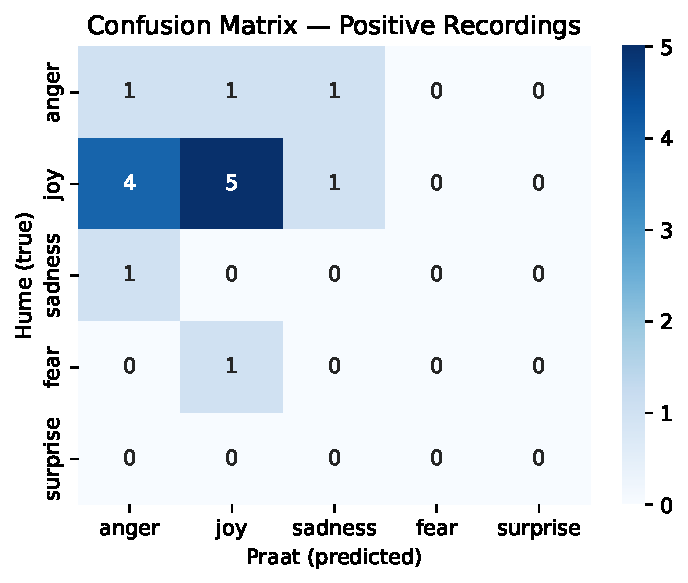
\includegraphics[width=\textwidth]{png/results/rq1_nr3/confusion_matrix_Positive_Recordings.pdf}
        \caption{Positive Recordings}
        \label{fig:rq1_conf_pos}
    \end{subfigure}
    \begin{subfigure}[b]{0.45\textwidth}
        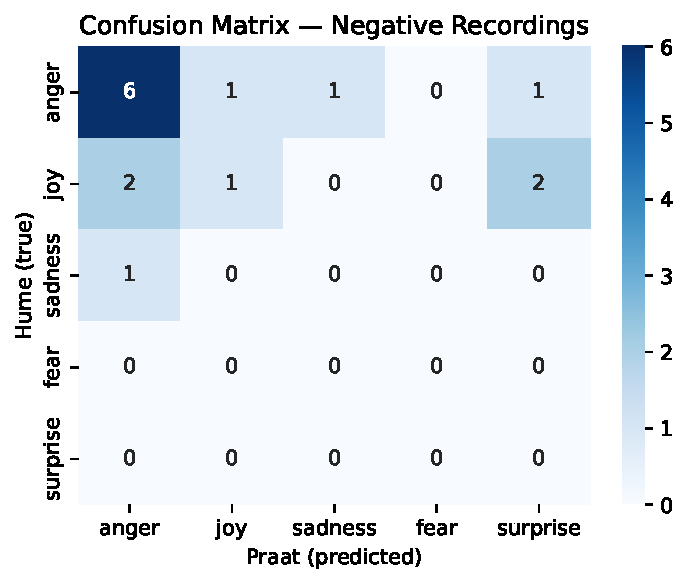
\includegraphics[width=\textwidth]{png/results/rq1_nr3/confusion_matrix_Negative_Recordings.pdf}
        \caption{Negative Recordings}
        \label{fig:rq1_conf_neg}
    \end{subfigure}
    \caption{Confusion matrix diagram for top label emotion between Hume and Custom Categorization.}
    \label{fig:rq1_conf_matx_full}
\end{figure}

The mean rated scores for Hume versus custom categorized emotion labels for positive recordings are illustrated in Figure~\ref{fig:rq1_scatter_custom_hume_pos}, negative in Figure~\ref{fig:rq1_scatter_custom_hume_neg}. As shown, some ratings follow the same pattern while other emotions diverge, as Hume joy are significantly higher for both sentiment categories while custom labelled surprise is overestimated compared to the Hume ranking. 
\begin{figure}[H]
    \centering 
    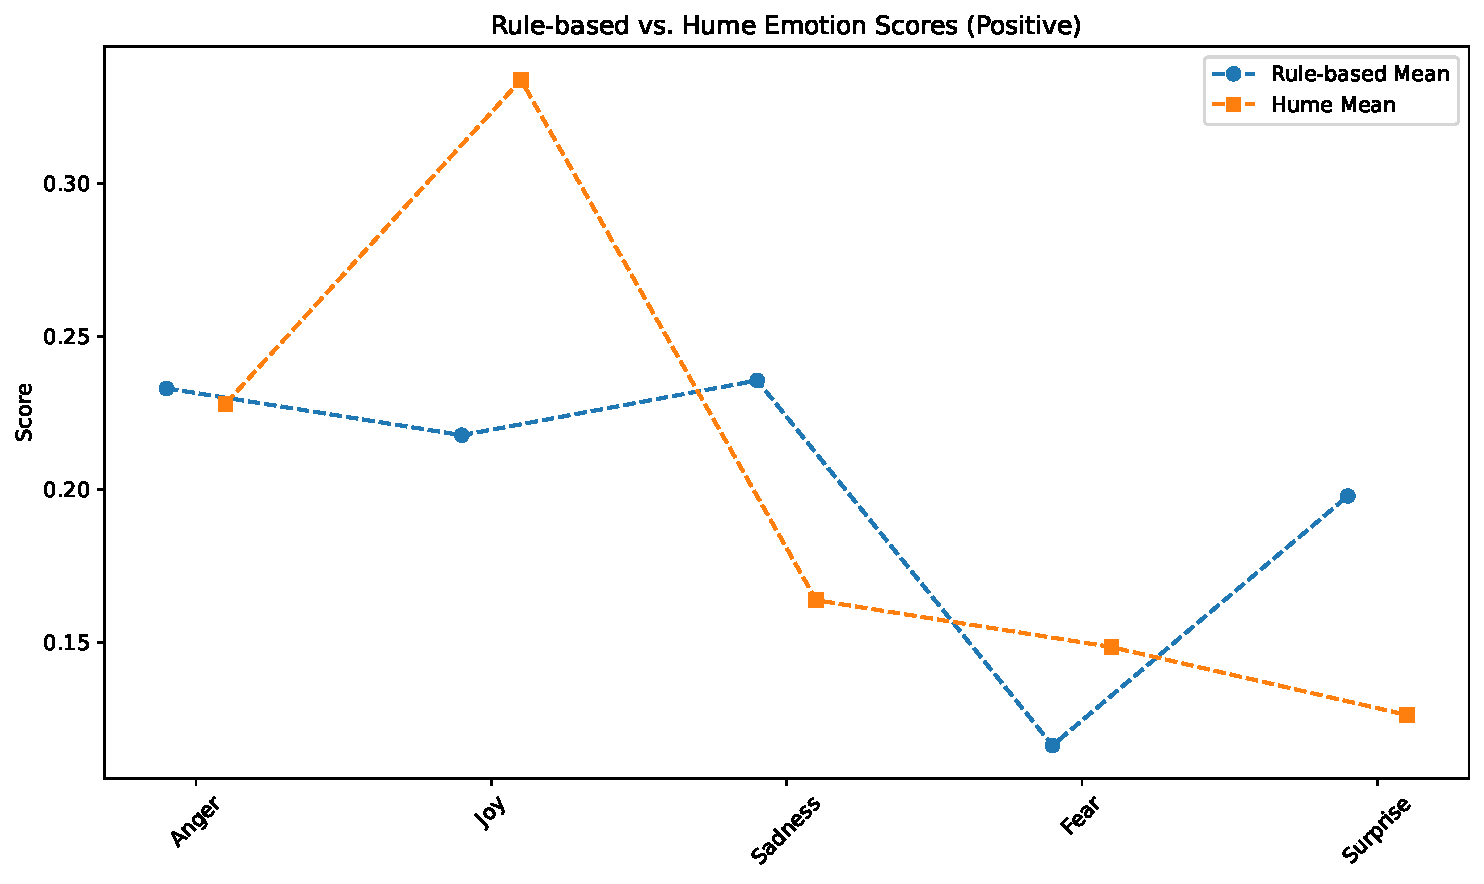
\includegraphics[width=0.7\textwidth]{png/results/rq1_nr3/praat_hume_positive_scatter.pdf}
    \caption{Scatter Plot of Mean Hume and Custom Emotion Scores, positive recordings.}
    \label{fig:rq1_scatter_custom_hume_pos}
\end{figure}

Custom labelled joy, sadness, and fear are ranked similarly in both positive and negative contexts. This pattern aligns with Hume probabilities that are more equal regarding surprise than the custom function for seperated sentiments. 
Anger is the most divergent emotion label across sentiments, with higher ratings in negative clips. Both sources rates anger, sadness, and fear relatively corresponding, Hume predicts anger slightly higher in negative contexts, while sadness is ranked lower than by the custom function for both sentiments. 
\begin{figure}[H]
    \centering 
    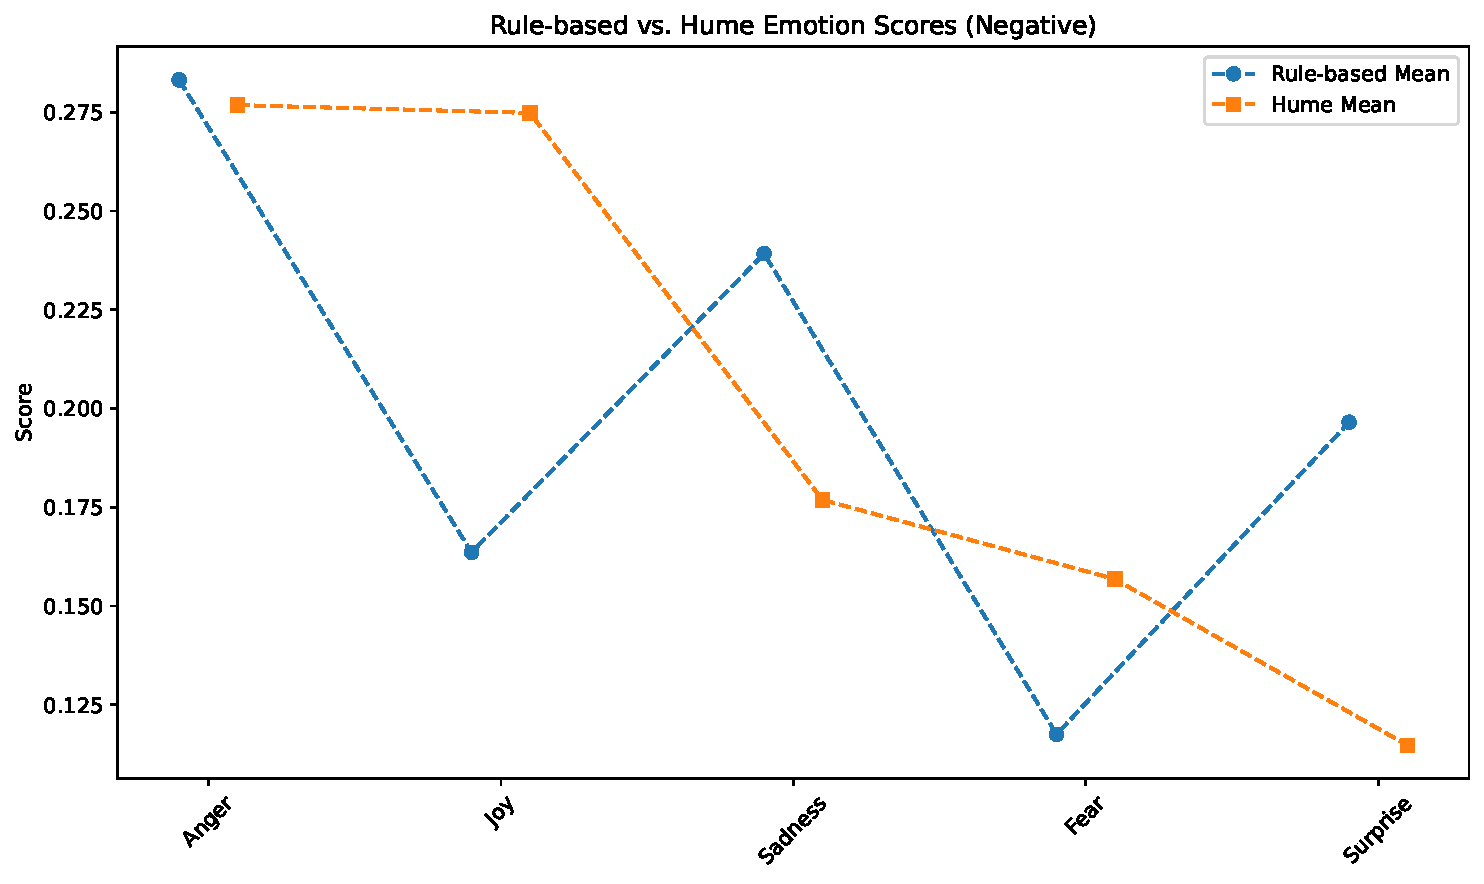
\includegraphics[width=0.7\textwidth]{png/results/rq1_nr3/praat_hume_negative_scatter.pdf}
    \caption{Scatter Plot of Mean Hume and Custom Emotion Scores, negative recordings.}
    \label{fig:rq1_scatter_custom_hume_neg}
\end{figure}


Pearson's correlation coefficients between Hume and custom categorized emotion labels are presented in Table~\ref{tab:rq1_corr_pos_neg_side_by_side} seperated by sentiment. 
Sadness in positive recordings is the single significant correlation (r = 9.614, p = 0.0149), other relationships remain weak. Correlations in the negative subset are slightly higher regarding the negative association with anger (r = -0.295. p = 0.2854) and a positive link with fear (r = 0.269, p = 0.3329), yet both of these correlations are weak without significance. 
All remaining labels presents near negligible correlation coefficients (r < 0.09). 


  \begin{table}[H]
    \centering
    \begin{subtable}{0.45\textwidth}
      \centering
      \caption*{\textbf{Positive Recordings}}
      \begin{tabular}{lrrl}
        \toprule
        \textbf{Emotion} & \textbf{Pearson’s r} & \textbf{p-value} & \textbf{Sign.} \\
        \midrule
        Anger      & -0.091        & 0.7474    & No          \\
        Joy        &  0.049        & 0.8613    & No          \\
        Sadness    &  0.614        & 0.0149    & Yes         \\
        Fear       & -0.044        & 0.8772    & No          \\
        Surprise   &  0.022        & 0.9375    & No          \\
        \bottomrule
      \end{tabular}
      \label{tab:rq1_corr_pos}
    \end{subtable}\hfill
    \begin{subtable}{0.45\textwidth}
      \centering
      \caption*{\textbf{Negative Recordings}}
      \begin{tabular}{lrrl}
        \toprule
        \textbf{Emotion} & \textbf{Pearson’s r} & \textbf{p-value} & \textbf{Sign.} \\
        \midrule
        Anger      & -0.295        & 0.2854    & No          \\
        Joy        & -0.029        & 0.9183    & No          \\
        Sadness    & -0.060        & 0.8330    & No          \\
        Fear       &  0.269        & 0.3329    & No          \\
        Surprise   & -0.081        & 0.7741    & No          \\
        \bottomrule
      \end{tabular}
      \label{tab:rq1_corr_neg}
    \end{subtable}
    \caption{Pearson’s r, p-values, and significance for positive vs.\ negative recordings.}
    \label{tab:rq1_corr_pos_neg_side_by_side}
  \end{table}
  
  

\subsection{Limitations of the Custom Vocal Emotion Categorization Method}

The rule-based function, customised to group emotions by vocal features as presented in the Swedish study \autocite{Ekberg2023}, often assigns equal top scores to multiple emotions for the same clip. 
The number of top rated emotion for separate recordings are summerised in Table~\ref{tab:rq1_number_rec_top}, showing that 60\% of the total clips have more than one top label for the custom function. By contrast, Hume has one singular top label for 29 of 30 clips. 
\begin{table}[H]
    \centering
    \begin{subtable}[t]{0.4\textwidth}
    
    \caption{Custom-categorisation}
    \begin{tabular}{l r r}
      \toprule
      \#Top Emotions & Clips & Percentage \\
      \midrule
      1               & 12         & 40\%       \\
      2               & 9          & 30\%       \\
      3               & 5          & 17\%       \\
      4               & 4          & 13\%       \\
      \bottomrule
    \end{tabular}
    \label{tab:praat_tie_summary}
  \end{subtable}
  \hfill
  \begin{subtable}[t]{0.4\textwidth}
    \caption{Hume AI}
    \label{tab:top_emotions_distribution_2}
    \begin{tabular}{lcc}
    \toprule
    \# Top Emotions & Clips & Percentage \\
    \midrule
    1               & 29         & 97\%       \\
    2               & 1          &  3\%       \\
    \bottomrule
    \end{tabular}
\end{subtable}
\caption{Distribution of recordings by number of top emotions}
\label{tab:rq1_number_rec_top}
\end{table}
    
To further demonstrate the occuring similarities in the emotion scoring by the rule-based function, bar charts for single clips is presented in Figure~\ref{fig:rq1_praat_hume_pos} for two seperate positive clips and Figure~\ref{fig:rq1_praat_hume_neg} illustrates two single negative interviews. 
Concurrence occurs for clip \ref{fig:praat_hume_008_pos}, for both Hume and the custom function except for joy that is predicted at high levels by Hume. 
Diagram \ref{fig:praat_hume_006_pos} and \ref{fig:praat_hume_009_neg} reveals reasonable approximation for certain emotions, as joy and fear in \ref{fig:praat_hume_006_pos} where Hume rates fear substantially higher. Similar pattern appears in \ref{fig:praat_hume_009_neg} for joy and sadness, in comparison to high predicted Hume-joy. 
However, discrepancies are presented in all single clips with varying dispersed. 
    

\begin{figure}[H]
    \centering
    \begin{subfigure}[t]{0.45\textwidth}
        \centering
        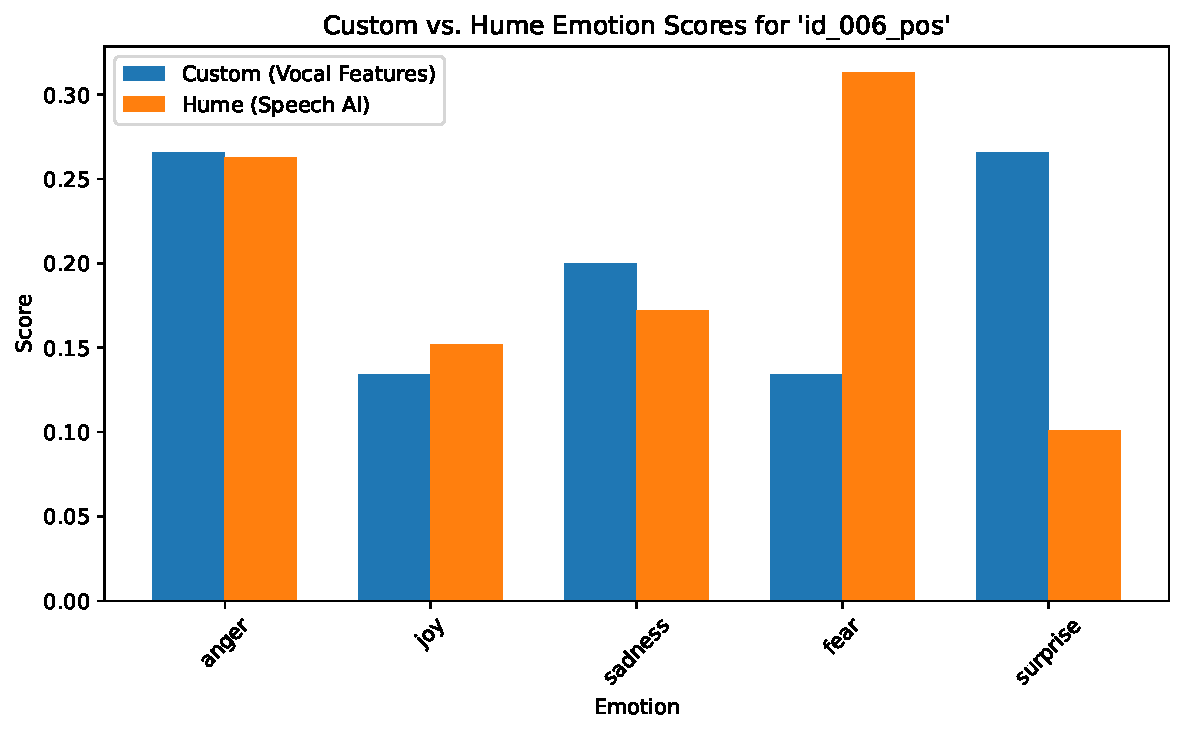
\includegraphics[width=0.9\textwidth]{png/results/rq1_nr3/id_006_pos_praat_hume_comparison.pdf}
        \caption{Single clip, female (id 006).}
        \label{fig:praat_hume_006_pos}
    \end{subfigure} 
    \begin{subfigure}[t]{0.45\textwidth}
        \centering
        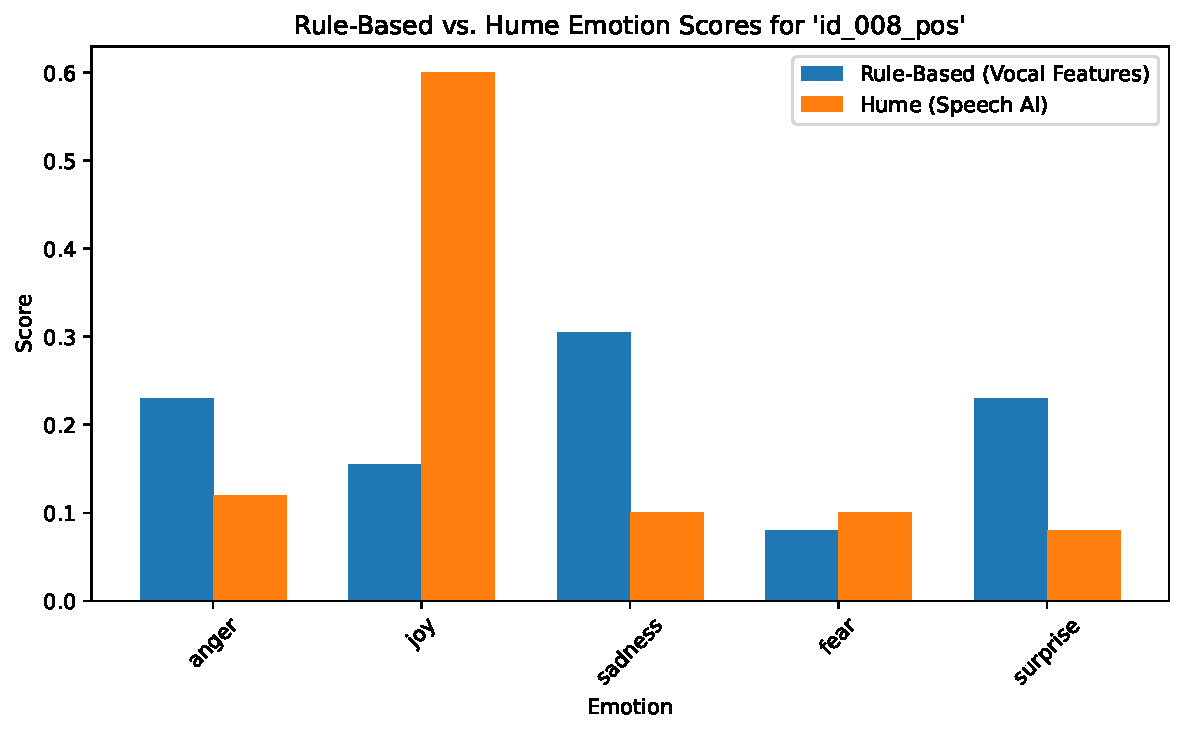
\includegraphics[width=0.9\textwidth]{png/results/rq1_nr3/id_008_pos_praat_hume_comparison.pdf}
        \caption{Single clip, male(id 008).}
        \label{fig:praat_hume_008_pos}
    \end{subfigure} 
    \caption{Custom emotion categorization vs. Hume for two seperate positive clips.}
    \label{fig:rq1_praat_hume_pos}
\end{figure}

\begin{figure}[H]
    \centering
    \begin{subfigure}[t]{0.45\textwidth}
        \centering
        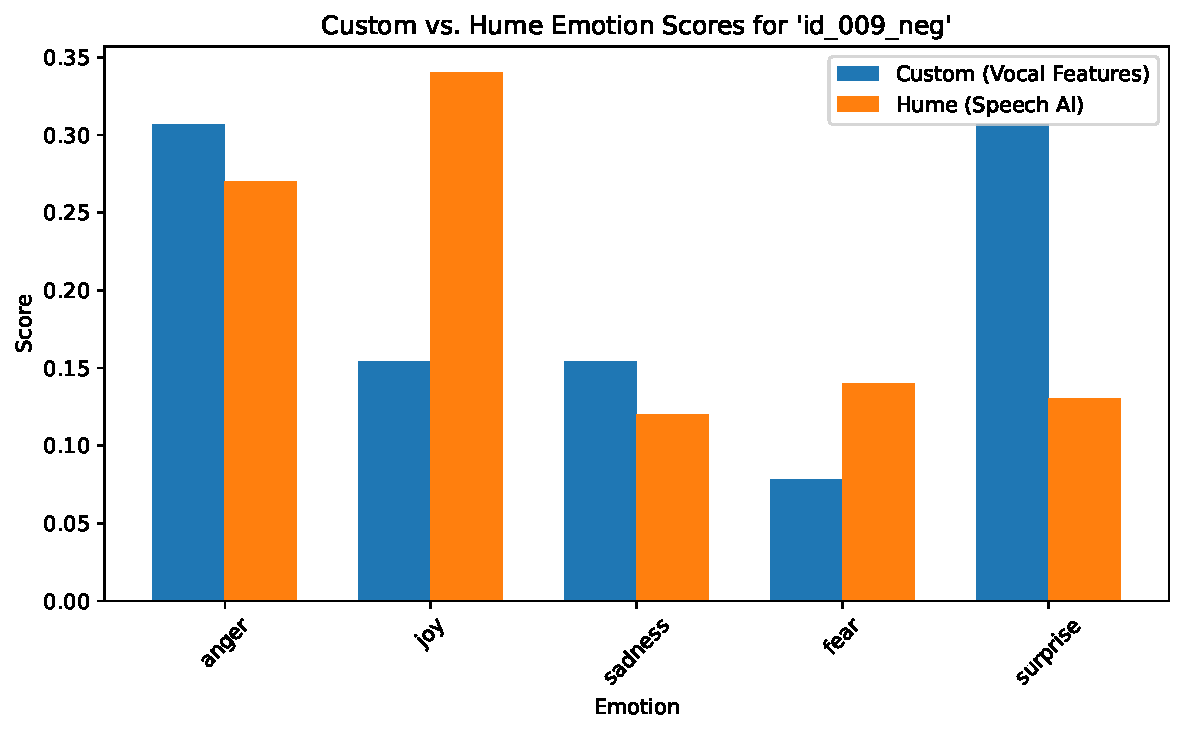
\includegraphics[width=0.9\textwidth]{png/results/rq1_nr3/id_009_neg_praat_hume_comparison.pdf}
        \caption{Single clip, female (id 009).}
        \label{fig:praat_hume_009_neg}
    \end{subfigure} 
    \begin{subfigure}[t]{0.45\textwidth}
        \centering
        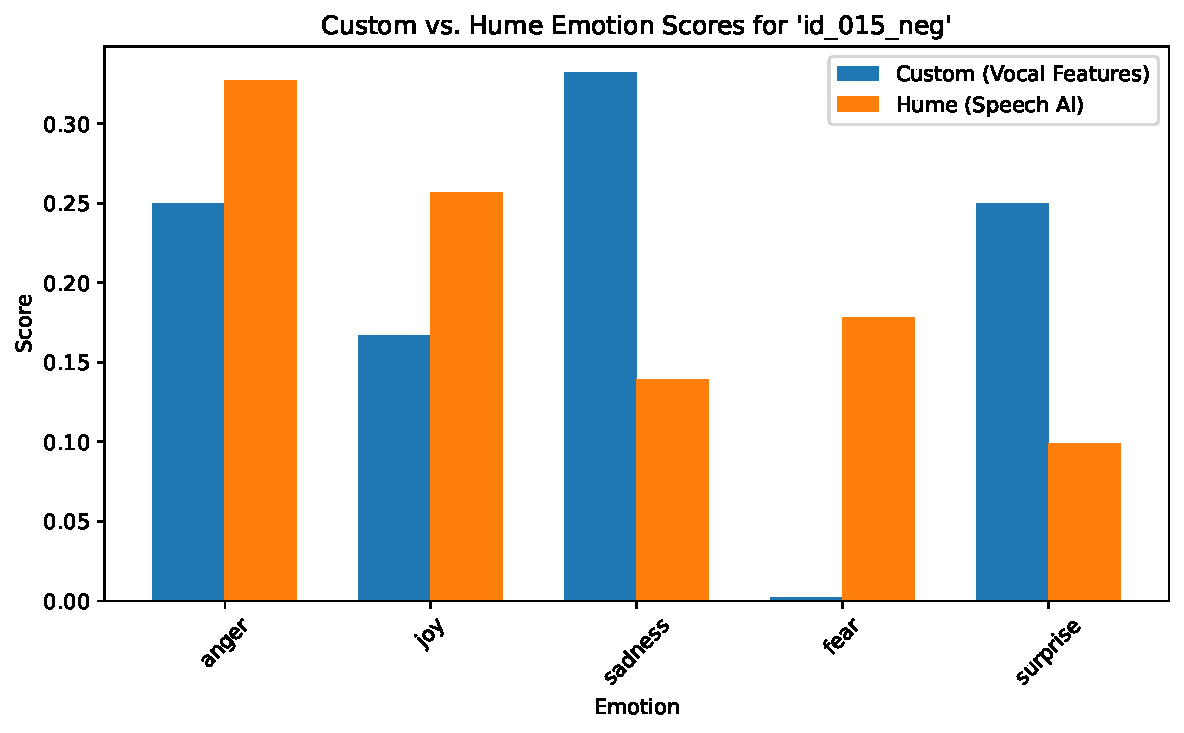
\includegraphics[width=0.9\textwidth]{png/results/rq1_nr3/id_015_neg_praat_hume_comparison.pdf}
        \caption{Single clip, male (id 015).}
        \label{fig:praat_hume_015_neg}
    \end{subfigure} 
    \caption{Custom emotion categorization vs. Hume for two seperate negative clips.}
    \label{fig:rq1_praat_hume_neg}
\end{figure}


\subsection{ANOVA Tables of Vocal Features Across Emotions}
An ANOVA was implemented to further examine whether essential vocal features varied across Hume-labelled emotions. This was conducted on mean values of full recordings for pitch, intensity, HNR, jitter, and shimmer. 
The results are summarised in Table~\ref{tab:rq1_anova_pos} for positive recordings and \ref{tab:rq1_anova_neg} for negative recordings, 
showing that none of the features showed statistically significant differences between the five Hume emotion categories (all p-values > 0.13, ranging up to > 0.90). 

\begin{table}[H]
    \centering 
    \begin{subtable}[b]{0.48\textwidth}
        \centering
        \caption*{\textbf{Positive recordings}}
        \begin{tabular}{lrr}
        \toprule
        \multicolumn{1}{c}{\textbf{Feature}} & \textbf{ANOVA P-value} & \textbf{Sign.} \\
        \midrule
        Pitch      & 0.7595    & No          \\
        Intensity  & 0.8627    & No          \\
        HNR        & 0.6149    & No          \\
        Jitter     & 0.9564    & No          \\
        Shimmer    & 0.7828    & No          \\
        \bottomrule
        \end{tabular}
        \caption{ANOVA: Positive recordings.}
        \label{tab:rq1_anova_pos}
    \end{subtable}
    \hfill
    \begin{subtable}[b]{0.48\textwidth}
        \centering
        \caption*{\textbf{Negative recordings}}
        \begin{tabular}{lrr}
        \toprule
        \multicolumn{1}{c}{\textbf{Feature}} & \textbf{ANOVA P-value} & \textbf{Sign.} \\
        \midrule
        Pitch      & 0.5393    & No          \\
        Intensity  & 0.1307    & No          \\
        HNR        & 0.5142    & No          \\
        Jitter     & 0.9066    & No          \\
        Shimmer    & 0.6863    & No          \\
        \bottomrule
        \end{tabular}
        \caption{ANOVA: Negative recordings.}
        \label{tab:rq1_anova_neg}
    \end{subtable}
    \caption{ANOVA for vocal features across emotions.}
    \label{tab:rq1_anova_all}
\end{table}  
  
These results imply that within our dataset of spontaneous speech during interviews, the average values of the acoustic features did not systematically vary according to AI-labeled emotions. 


\subsection{Time-to-Time Analysis}


\subsubsection{Time-to-Time Analysis: Full Dataset}
To understand both if acoustic cues correlates with emotion probability by Hume and when they produce clear categorical shifts, two analyses were conducted at time segmened level. 
These effects were observed further with sentiment seperations of all, negative, and positive contexts to see if the emotion-acoustic feature relationship are dependent on positive vs. negative sentiment. 
Table \ref{tab:rq1_time_all_correlations} presents the significant correlations between z-scored acoustic features and Hume emotions.
\begin{table}[H]
    \centering
    %\caption*{\textbf{All Recordings}}
    \begin{tabular}{l l r r l}
      \toprule
      \textbf{Feature} & \textbf{Emotion} & \textbf{Pearson’s r} & \textbf{p-value} & \textbf{Significant} \\
      \midrule
        pitch      & joy     & 0.065         & 0.0448    & Yes         \\
        pitch      & sadness & -0.230        & 0.0000    & Yes         \\
        pitch      & fear    & 0.082         & 0.0110    & Yes         \\
        intensity  & joy     & 0.164         & 0.0000    & Yes         \\
        intensity  & sadness & -0.142        & 0.0000    & Yes         \\
        intensity  & fear    & -0.173        & 0.0000    & Yes         \\
        intensity  & surprise& -0.110        & 0.0006    & Yes         \\
        HNR        & sadness & -0.253        & 0.0000    & Yes         \\
        HNR        & fear    & 0.112         & 0.0005    & Yes         \\
        jitter     & sadness & 0.084         & 0.0091    & Yes         \\
      \bottomrule
    \end{tabular}
    \caption{Significant Pearson correlations for the full dataset.}
    \label{tab:rq1_time_all_correlations}
  \end{table}
 
  Only significant correlation is included (all p < 0.05). 9 correlations out of 24 indicated significance, the full analysis is presented in Appendix [FIGURE REF]. 
  All correlations are perceived as weak even if there is statistical significance. Pitch correlated positively with joy (r = 0.065), negatively with sadness (r = -0.230) and positive with fear (r = 0.082). 
  Intensity had a increased relationship with joy (r = 0.164), but decreased with sadness (r = -0.142), fear (r = -0.173) and surprise (r = -0.110). 
  HNR showed a weak negative correlation with sadness (r = -0.253) and positive with fear (r = 0.112). 
  Jitter had a single significant, yet weak correlation with sadness (r = 0.084). Shimmer showed no significant correlations. 

\medskip
Table \ref{tab:ttest_full_features} compares the top 30\% and bottom 70\% of emotion-probability time-segments, and tests wheather the mean z-scored feature differs between the high vs. low groups. 
A large t-statistic value indicate a reliable shift in that feature when Hume rates that emotion high. 
\begin{table}[H]
    \centering
    \begin{tabular}{l l r r l}
      \toprule
      \textbf{Feature} & \textbf{Emotion} & \textbf{t-statistic} & \textbf{p-value} & \textbf{Significant} \\
      \midrule
        pitch X     & anger   &  2.529      & 0.0116    & Yes         \\
        pitch       & joy     &  2.293      & 0.0221    & Yes         \\
        pitch       & sadness & -7.769      & 0.0000    & Yes         \\
        pitch       & fear    &  5.185      & 0.0000    & Yes         \\
        intensity X & anger   &  1.975      & 0.0485    & Yes         \\
        intensity   & joy     &  4.602      & 0.0000    & Yes         \\
        intensity   & sadness & -3.981      & 0.0001    & Yes         \\
        intensity   & fear    & -3.567      & 0.0004    & Yes         \\
        intensity   & surprise& -2.949      & 0.0033    & Yes         \\
        HNR         & anger   &  2.709      & 0.0069    & Yes         \\
        HNR         & sadness & -7.506      & 0.0000    & Yes         \\
        HNR         & fear    &  4.914      & 0.0000    & Yes         \\
        HNR X       & surprise&  2.287      & 0.0224    & Yes         \\
        jitter      & sadness &  1.811      & 0.0705    & No          \\
      \bottomrule
    \end{tabular}
    \caption{High-vs-low t-test results for significant acoustic features (full dataset)}
    \label{tab:ttest_full_features}
  \end{table}
  
  High-anger predictions of segmented recordings had higher pitch (t = 2.529), intensity (t = 1.975) and HNR (t = 2.709), none of these associations was significant in the data for Table~\ref{tab:rq1_time_all_correlations}. 
  Joy segments had increased pitch (t = 2.293) and intensity (t = 4.602), while fear segments have lower intensity (t = -3.567) and increased pitch (t = 5.185) and HNR (t = 4.914). 
  High-sadness segments showed notable decreased pitch (t = -7.769), intensity (t = -3.981), HNR (t = -7.506), and a small, not significant increase in jitter (t = 1.811, p = 0.0705).
  Segments with high surprise predictions has the moderately low intensity (t = -2.949) and a modest positive differention for HNR (t = 2.287). 
  

  \subsubsection{Time-to-Time Analysis by Sentiment}
  \begin{table}[H]
    \centering
    \begin{subtable}{0.45\textwidth}
      \centering
      \caption{Pitch and Anger (Pearson r)}\label{tab:rq1_corr_pitch_anger}
      \begin{tabular}{l r r l}
        \toprule
        Sentiment & \(\;r\;\) & \(\;p\;\) & Sign. \\
        \midrule
        All        &  0.032        & 0.3284    & No          \\
        Positive   & -0.042        & 0.3772    & No          \\
        Negative   &  0.101        & 0.0209    & Yes         \\
        \bottomrule
      \end{tabular}
    \end{subtable}\hfill
    \begin{subtable}{0.45\textwidth}
      \centering
      \caption{Pitch and Anger (t-test)}\label{tab:rq1_ttest_pitch_anger}
      \begin{tabular}{l r r l}
        \toprule
        Sentiment & \(\;t\;\) & \(\;p\;\) & Sign. \\
        \midrule
        All        &  2.529      & 0.0116    & Yes         \\
        Positive   &  1.392      & 0.1647    & No          \\
        Negative   &  2.642      & 0.0085    & Yes         \\
        \bottomrule
      \end{tabular}
    \end{subtable}
    \caption{(a) Pearson correlations and (b) high-vs-low t-test results for pitch vs. anger by sentiment.}
    \label{tab:rq1_pitch_anger_side_by_side}
  \end{table}
  
  Table \ref{tab:rq1_pitch_anger_side_by_side} presents an absent correlation between pitch and anger for the full dataset (r = 0.032, p = 0.3284), and positive clips (r = -0.042, p = 0.3772) but a significant, yet weak correlation in the negative subset (r = 0.101, p = 0.0209). 
  The t-tests in \ref{tab:rq1_ttest_pitch_anger} confirms this where high-anger segments have moderate higher pitch in the negative set (t = 2.642, p = 0.0085) and in for all clips (t = 2.529, p = 0.0116), but not in positive contexts. 
  This implies that pitch is a considerable signal of anger when the overall context is negative. 

  \begin{table}[H]
    \centering
  
    %%% HNR ⇔ Anger block %%%
    \begin{subtable}{0.45\textwidth}
      \centering
      \caption{HNR and Anger (r)}\label{tab:rq1_corr_hnr_anger}
      \begin{tabular}{l r r l}
        \toprule
        Sentiment & \(\;r\;\) & \(\;p\;\) & Sign. \\
        \midrule
        All        &  0.059        & 0.0695    & No          \\
        Positive   & -0.001        & 0.9750    & No          \\
        Negative   &  0.111        & 0.0109    & Yes         \\
        \bottomrule
      \end{tabular}
    \end{subtable}\hfill
    \begin{subtable}{0.45\textwidth}
      \centering
      \caption{HNR and Anger (t-test)}\label{tab:rq1_ttest_hnr_anger}
      \begin{tabular}{l r r l}
        \toprule
        Sentiment & \(\;t\;\) & \(\;p\;\) & Sign. \\
        \midrule
        All        &  2.709      & 0.0069    & Yes         \\
        Positive   &  1.941      & 0.0529    & No          \\
        Negative   &  3.123      & 0.0019    & Yes         \\
        \bottomrule
      \end{tabular}
    \end{subtable}
  
    \caption{HNR–Anger correlations and t-test results by sentiment.}
    \label{tab:rq1_hnr_anger_side_by_side}
  \end{table}
  
  Table \ref{tab:rq1_hnr_anger_side_by_side} presents harmonic-to-noise correlation with anger for the full dataset (r = 0.059, p = 0.695), implying an unsignificant weak correlation.  
  T-tests in \ref{tab:rq1_ttest_hnr_anger} shows that HNR slightly distinguish high vs low anger for both the full and negative dataset (t = 2.709, t = 3.123 respectively).
  These correlations is significantly weak, in negative contexts (r = 0.111, p = 0.0109) but non-significant in positive recordings (r = -0.001, p = 0.9750), which also has a non-significant distinction in the t-tests.
  Together with pitch, HNR appears to be the most prevalent features correlated with anger in negative circumstances, even if the shifts in vocal features for this emotion is fairly weak. 
  
  \begin{table}[H]
    \centering
  
    %%% Pitch ⇔ Joy block %%%
    \begin{subtable}{0.45\textwidth}
      \centering
      \caption{Pitch and Joy (r)}\label{tab:rq1_corr_pitch_joy}
      \begin{tabular}{l r r l}
        \toprule
        Sentiment & \(\;r\;\) & \(\;p\;\) & Sign. \\
        \midrule
        All        & 0.065         & 0.0448    & Yes         \\
        Positive   & 0.110         & 0.0210    & Yes         \\
        Negative   & 0.014         & 0.7567    & No          \\
        \bottomrule
      \end{tabular}
    \end{subtable}\hfill
    \begin{subtable}{0.45\textwidth}
      \centering
      \caption{Pitch and Joy (t-test)}\label{tab:rq1_ttest_pitch_joy}
      \begin{tabular}{l r r l}
        \toprule
        Sentiment & \(\;t\;\) & \(\;p\;\) & Sign. \\
        \midrule
        All        & 2.293        & 0.0221    & Yes         \\
        Positive   & 1.816        & 0.0701    & No          \\
        Negative   & 0.617        & 0.5374    & No          \\
        \bottomrule
      \end{tabular}
    \end{subtable}
  
    \caption{Pitch–Joy correlations and t-test results by sentiment.}
    \label{tab:rq1_pitch_joy_side_by_side}
  \end{table}
  
  Pitch and joy correlations is presented in Table~\ref{tab:rq1_pitch_joy_side_by_side}, showing unlike anger, a weak correlation for the full dataset (r = 0.065, p = 0.0448). 
  Pitch reaches a weak correlation with joy in positive recordings (r = 0.110, p = 0.0210) and no significance in the negative subset. 
  The t-tests is only significant in the full dataset (t = 2.293, p = 0.0221), not for the positive clips (t = 1.861, p = 0.0701), implying a more context-specific and non-linear affect.
  
  \begin{table}[H]
    \centering
  
    %%% Intensity ⇔ Joy block %%%
    \begin{subtable}{0.45\textwidth}
      \centering
      \caption{Intensity and Joy (r)}\label{tab:rq1_corr_intensity_joy}
      \begin{tabular}{l r r l}
        \toprule
        Sentiment & \(\;r\;\) & \(\;p\;\) & Sign. \\
        \midrule
        All        & 0.164        & 0.0000    & Yes         \\
        Positive   & 0.175        & 0.0002    & Yes         \\
        Negative   & 0.152        & 0.0005    & Yes         \\
        \bottomrule
      \end{tabular}
    \end{subtable}\hfill
    \begin{subtable}{0.45\textwidth}
      \centering
      \caption{Intensity and Joy (t-test)}\label{tab:rq1_ttest_intensity_joy}
      \begin{tabular}{l r r l}
        \toprule
        Sentiment & \(\;t\;\) & \(\;p\;\) & Sign. \\
        \midrule
        All        & 4.602        & 0.0000    & Yes         \\
        Positive   & 3.343        & 0.0009    & Yes         \\
        Negative   & 2.375        & 0.0179    & Yes         \\

        \bottomrule
      \end{tabular}
    \end{subtable}
  
    \caption{Intensity–Joy correlations and t-test results by sentiment.}
    \label{tab:rq1_intensity_joy_side_by_side}
  \end{table}
Table \ref{tab:rq1_intensity_joy_side_by_side} demonstrates the correlation between intensity and joy, showing stronger associations compared to joy and pitch. 
All contexts show a positive relationship, strongest for positive clips (r = 0.175, p = 0.0002) with significant mean differences where the full dataset has highest significance (t = 4.602, p < 0.001). 
These results suggests that intensity is a reasonably stable cue to joy regardless of the overall sentiment context, even if higher correlation occurs for the full and positive sets than the negative subset (r = 0.152 and t = 2.375). 

\begin{table}[H]
    \centering
  
    %%% pitch and sadness block %%%
    \begin{subtable}{0.45\textwidth}
      \centering
      \caption{Pitch and Sadness (r)}\label{tab:rq1_corr_pitch_sadness}
      \begin{tabular}{l r r l}
        \toprule
        Sentiment & \(\;r\;\) & \(\;p\;\) & Sign. \\
        \midrule
        All        & -0.230        & 0.0000    & Yes         \\
        Positive   & -0.275        & 0.0000    & Yes         \\
        Negative   & -0.187        & 0.0000    & Yes         \\
        \bottomrule
      \end{tabular}
    \end{subtable}\hfill
    \begin{subtable}{0.45\textwidth}
      \centering
      \caption{Pitch and Sadness (t-test)}\label{tab:rq1_ttest_pitch_sadness}
      \begin{tabular}{l r r l}
        \toprule
        Sentiment & \(\;t\;\) & \(\;p\;\) & Sign. \\
        \midrule
        All        & -7.769       & 0.0000    & Yes         \\
        Positive   & -6.332       & 0.0000    & Yes         \\
        Negative   & -4.980       & 0.0000    & Yes         \\
        \bottomrule
      \end{tabular}
    \end{subtable}
  
    \caption{Pitch–Sadness correlations and t-test results by sentiment.}
    \label{tab:rq1_pitch_sadness_side_by_side}
  \end{table}
  
  Table \ref{tab:rq1_pitch_sadness_side_by_side} display seperated sentiment correlations for pitch and Hume predicted sadness, with significant difference between high and low groups indicating prominent shifts in pitch when Hume rates sadness high. 
  Correlations are weak, but significant for all sentiment contexts. Positive recordings show the largest negative correlation (r = -0.275, p < 0.001), although the full dataset reveals greater diverge in variations (t = -7.769, p < 0.001). 
  The negative subset accommodate lowest correlation and shifts in pitch for sadness.     
  
  \begin{table}[H]
    \centering
  
    %%% Intensity ⇔ Joy block %%%
    \begin{subtable}{0.45\textwidth}
      \centering
      \caption{HNR and Sadness (r)}\label{tab:rq1_corr_hnr_sadness}
      \begin{tabular}{l r r l}
        \toprule
        Sentiment & \(\;r\;\) & \(\;p\;\) & Sign. \\
        \midrule
        All        & -0.253        & 0.0000    & Yes         \\
        Positive   & -0.243        & 0.0000    & Yes         \\
        Negative   & -0.262        & 0.0000    & Yes         \\
        \bottomrule
      \end{tabular}
    \end{subtable}\hfill
    \begin{subtable}{0.45\textwidth}
      \centering
      \caption{HNR and Sadness (t-test)}\label{tab:rq1_ttest_hnr_sadness}
      \begin{tabular}{l r r l}
        \toprule
        Sentiment & \(\;t\;\) & \(\;p\;\) & Sign. \\
        \midrule
        All        & -7.506       & 0.0000    & Yes         \\
        Positive   & -5.442       & 0.0000    & Yes         \\
        Negative   & -5.049       & 0.0000    & Yes         \\

        \bottomrule
      \end{tabular}
    \end{subtable}
  
    \caption{HNR-Sadness correlations and t-test results by sentiment.}
    \label{tab:rq1_hnr_sadness_side_by_side}
  \end{table}

HNR showed to be an indicator of sadness in Table \ref{tab:ttest_full_features} and \ref{tab:rq1_time_all_correlations}, presented further in Table \ref{tab:rq1_hnr_sadness_side_by_side}. The patterns between sadness and HNR is similar to pitch, such that significant correlation occur across all sentiments with large differentions in HNR fluctuation. 
Negative conditions show strongest negative correlation (r = -0.262, p < 0.001), followed by the full dataset (r = -0.253, p < 0.001) that exhibit the largest variations of vocal variance regarding sadness (t = -7.506, p < 0.001). 

These large t-statistics suggests that reduced pitch and HNR are indicators of sadness independent from sentiment orientation. 

\subsubsection{Case Examples}
For a more concrete illustration of the prior tendencies , three interview recordings were analyzed in detail. The purpose was to examine whether emotional shifts become more apparent when evaluating shorter time segments within individual speakers, compared to the weaker correlations observed at the dataset level.

\medskip

\begin{figure}[H]
    \centering
    
    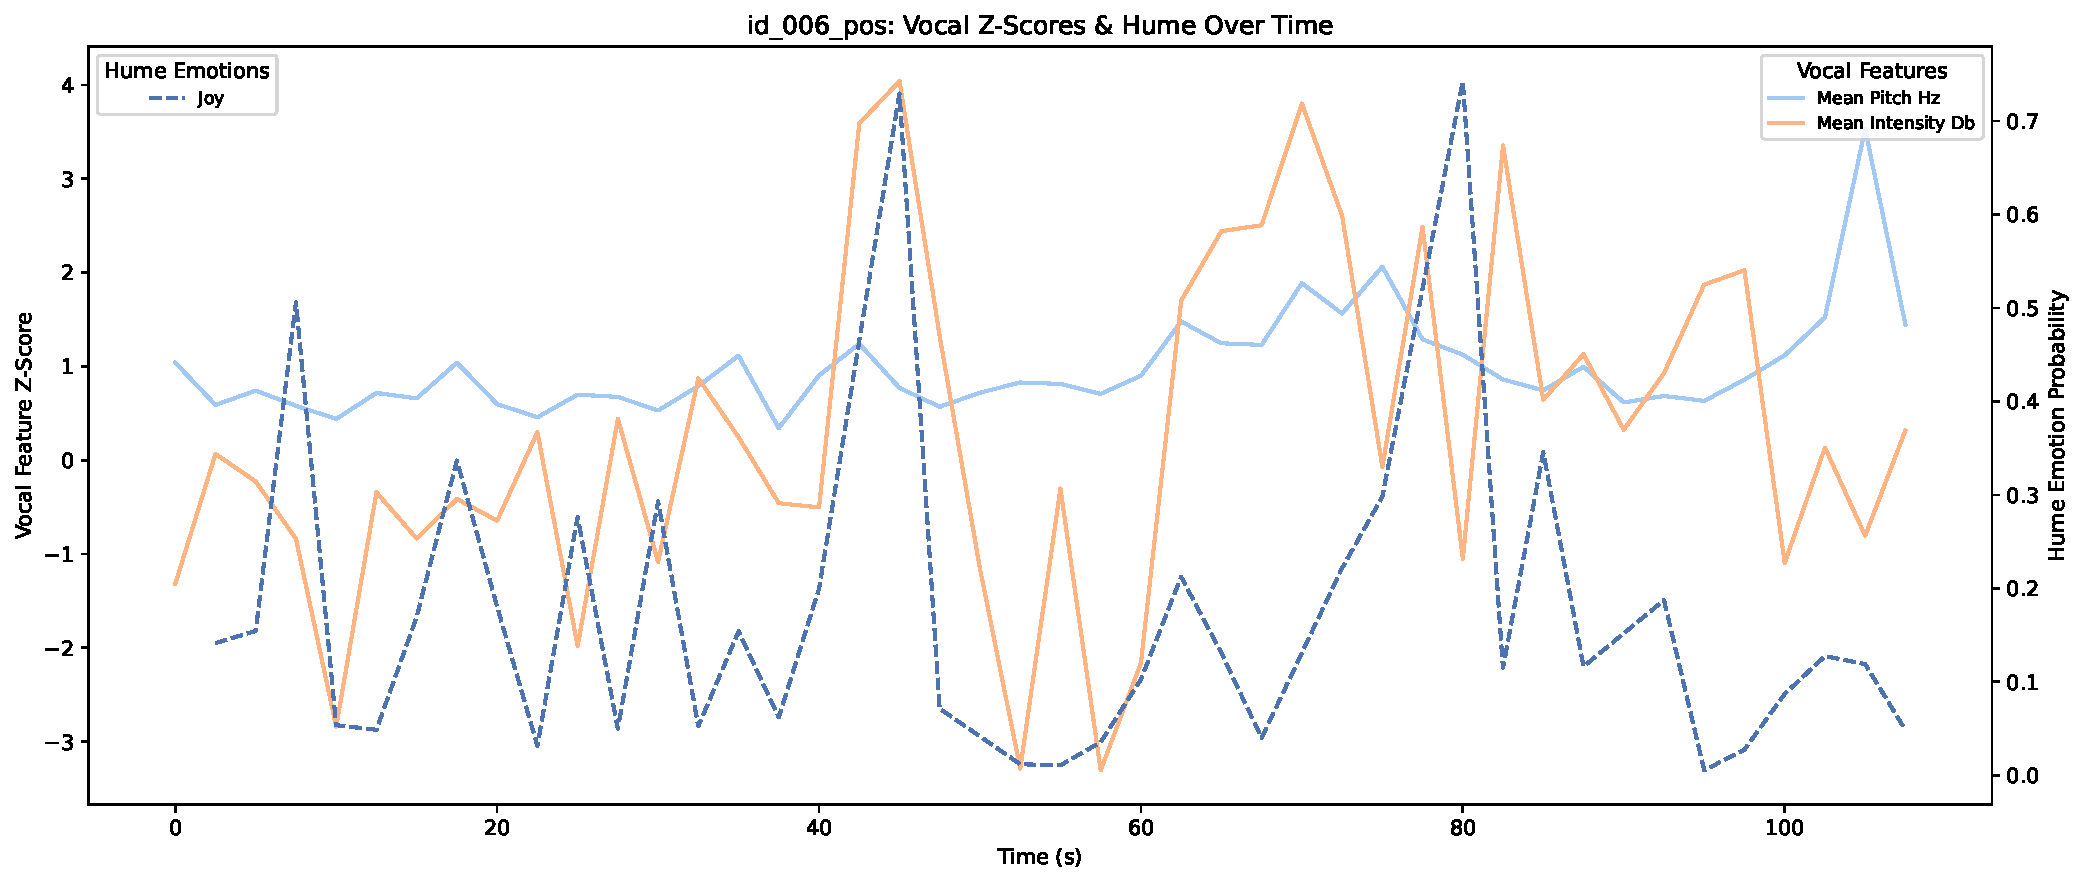
\includegraphics[width=0.85\textwidth]{png/results/rq3_2/combined_zscore_hume_id_006_pos_4.pdf}
    \caption{Pitch and Intensity vs. Hume Joy for single positive clip.}
    \label{fig:006_pos-joy}
\end{figure}

\begin{table}[ht]
    \centering
    \begin{subtable}[t]{0.48\textwidth}
      \centering
      \caption{Pearson Correlation (Clip id\_006\_pos)}
      \label{tab:clip006_pos_pearson}
      \begin{tabular}{llrrl}
        \toprule
        Feature            & Emotion &  $r$ & $p$ & Sign \\
        \midrule
        pitch\     & joy     &  0.188        & 0.1965    & No  \\
        intensity & joy     &  0.351        & 0.0134    & Yes \\
        intensity & fear    & -0.413        & 0.0032    & Yes \\
        jitter      & fear    & -0.291        & 0.0426    & Yes \\
        \bottomrule
      \end{tabular}
    \end{subtable}
    \hfill
    \begin{subtable}[t]{0.48\textwidth}
      \centering
      \caption{t-test (Clip id\_006\_pos)}
      \label{tab:clip006_pos_ttest}
      \begin{tabular}{llrrl}
        \toprule
        Feature            & Emotion & t & $p$ & Sign \\
        \midrule
        pitch     & joy     &  0.331       & 0.7419    & No  \\
        intensity & joy     &  2.718       & 0.0092    & Yes \\
        \bottomrule
      \end{tabular}
    \end{subtable}
    \caption{Statistical results for clip id\_006\_pos}
    \label{tab:clip006_pos_stats}
  \end{table}
  
% ----------------- Clip ID 006 -----------------
% \begin{table}[H]
%     \centering
%     \begin{subtable}{0.45\textwidth}
%       \centering
%       \caption{Correlation (ID 006)}\label{tab:id006_corr}
%       \begin{tabular}{l r r r}
%         \toprule
%         \textbf{Feature} & \textbf{Emotion} & \textbf{\(r\)} & \textbf{Sign.} \\
%         \midrule
%         pitch     & surprise &  0.365 & Yes \\
%         intensity & anger    &  0.333 & Yes \\
%         intensity & fear     & –0.415 & Yes \\
%         \bottomrule
%       \end{tabular}
%     \end{subtable}\hfill
%     \begin{subtable}{0.45\textwidth}
%       \centering
%       \caption{High vs Low T-Test (ID 006)}\label{tab:id006_ttest}
%       \begin{tabular}{l l r r r}
%         \toprule
%         \textbf{Feature} & \textbf{Emotion} & \textbf{t} & \textbf{p} & \textbf{Sign.} \\
%         \midrule
%         pitch     & surprise &  2.622 & 0.0121 & Yes \\
%         intensity & anger    &  2.333 & 0.0245 & Yes \\
%         intensity & fear     & –1.629 & 0.1109 & No  \\
%         \bottomrule
%       \end{tabular}
%     \end{subtable}
  
%     \caption{ID 006: Pearson correlations and high-vs-low t-tests for key features.}
%     \label{tab:id006_summary}
%   \end{table}

\textbf{24 rows for all!!! }
\begin{figure}[H]
    \centering
    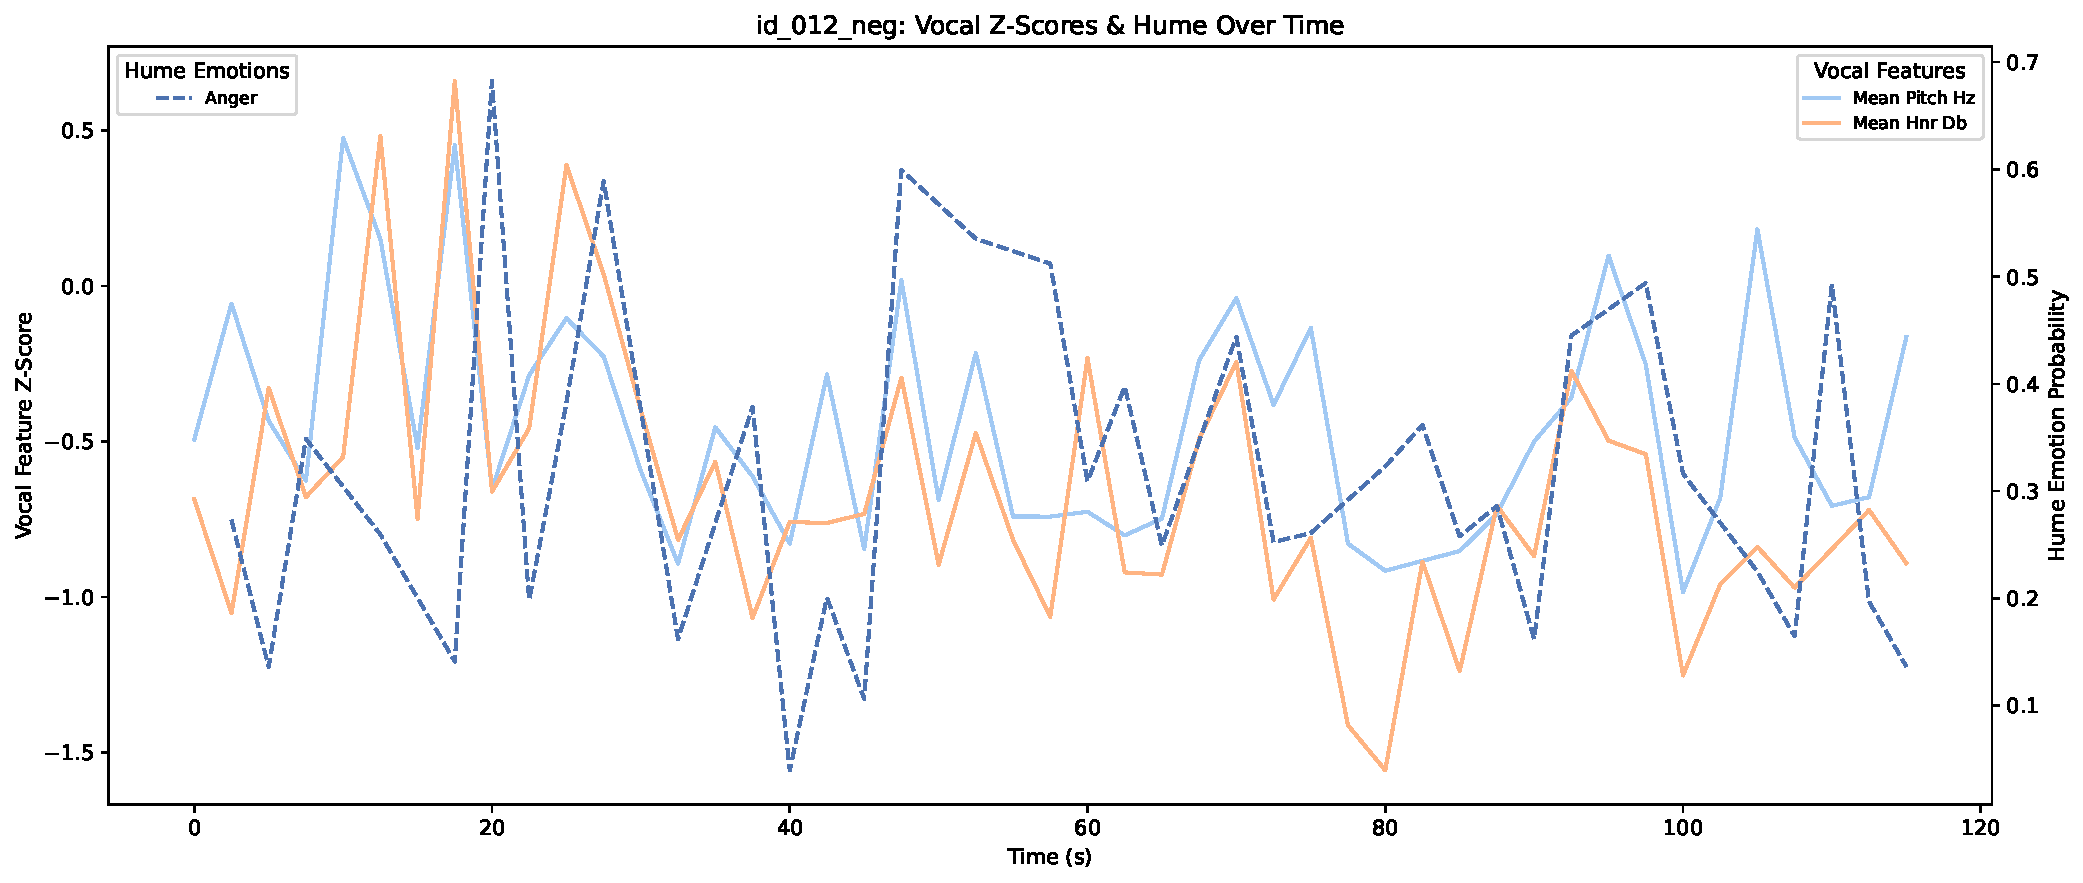
\includegraphics[width=0.85\textwidth]{png/results/rq3_2/combined_zscore_hume_id_012_neg_6.pdf} 
    \caption{Pitch and HNR vs. Hume Anger for single negative clip.}
    \label{fig:012_neg-anger}
\end{figure}

\begin{table}[ht]
    \centering
    \begin{subtable}[t]{0.48\textwidth}
      \centering
      \caption{Clip id\_012\_neg – Pearson Correlation}
      \label{tab:clip012_pearson}
      \begin{tabular}{lllrrl}
        \toprule
        Feature               & Emotion & $r$ & $p$ & Sign \\
        \midrule
        pitch       & fear    &  0.393 & 0.0122 & Yes  \\
        intensity    & fear    & -0.465 & 0.0025 & Yes  \\
        hnr          & anger   & -0.114 & 0.4846 & No \\
        hnr          & fear    &  0.437 & 0.0048 & Yes  \\
        shimmer        & sadness & -0.354 & 0.0248 & Yes  \\
        shimmer         & fear    & -0.356 & 0.0240 & Yes  \\
        \bottomrule
      \end{tabular}
    \end{subtable}
    \hfill
    \begin{subtable}[t]{0.48\textwidth}
      \centering
      \caption{Clip id\_012\_neg – t-test}
      \label{tab:clip012_ttest}
      \begin{tabular}{lllrrl}
        \toprule
        Feature               & Emotion & t & $p$& Sign \\
        \midrule
        pitch        & anger   & -0.353 & 0.7259 & No \\
        pitch        & fear    &  2.700 & 0.0103 & Yes  \\
        intensity    & anger   &  2.255 & 0.0300 & Yes  \\
        hnr          & anger   &  0.880 & 0.3844 & No \\
        \bottomrule
      \end{tabular}
    \end{subtable}
    \caption{Statistical results for clip id\_012\_neg}
    \label{tab:clip012_stats}
  \end{table}

\begin{figure}[H]
    \centering
    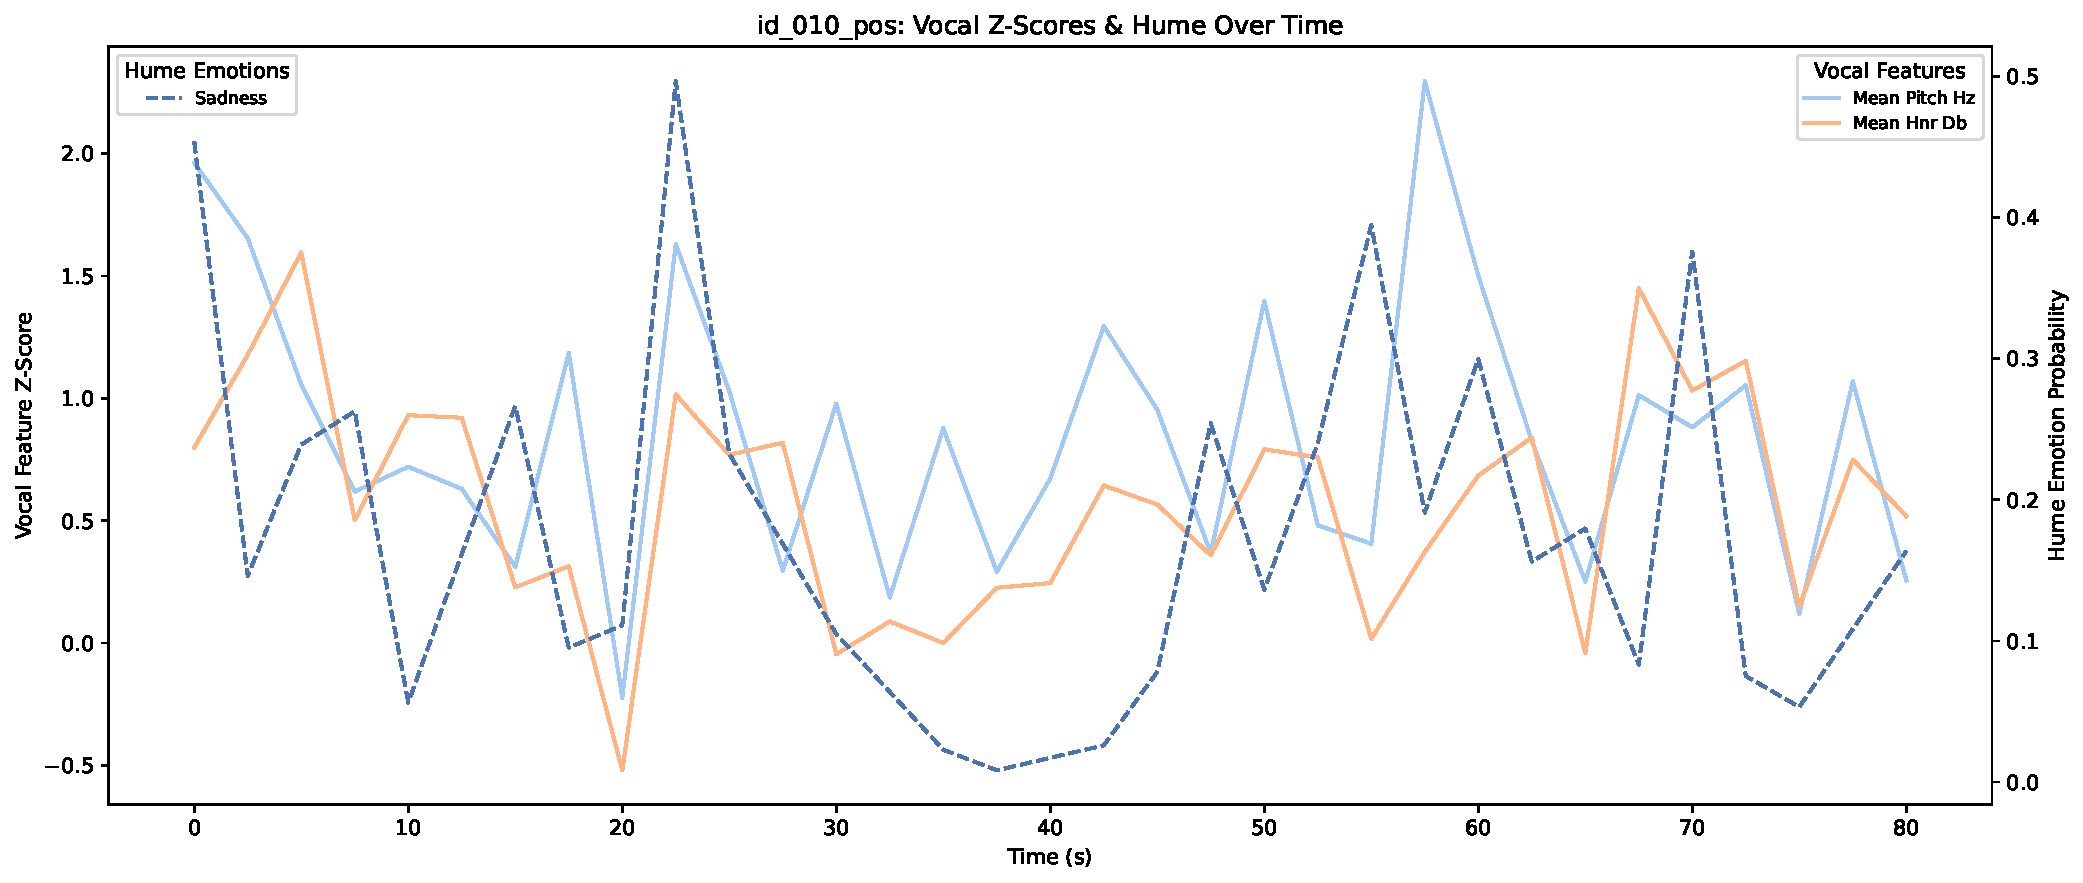
\includegraphics[width=0.85\textwidth]{png/results/rq1_nr3/combined_zscore_hume_id_010_pos_7.pdf}
    \caption{Pitch and HNR vs. Hume Sadness for single positive clip.}
    \label{fig:010_pos-sadness}
\end{figure}

\begin{table}[ht]
    \centering
    \begin{subtable}[t]{0.48\textwidth}
      \centering
      \caption{Clip id\_010\_pos – Pearson Correlation}
      \label{tab:clip010_pos_pearson}
      \begin{tabular}{lllrrl}
        \toprule
        Feature            & Emotion  & $r$ & $p$ & Sign \\
        \midrule
        mean\_pitch\_hz     & sadness  & -0.032        & 0.8632    & No          \\
        mean\_pitch\_hz     & fear     &  0.399        & 0.0260    & Yes         \\
        mean\_pitch\_hz     & surprise &  0.383        & 0.0332    & Yes         \\
        mean\_hnr\_db       & sadness  & -0.149        & 0.4225    & No          \\
         mean\_hnr\_db       & fear     &  0.389        & 0.0306    & Yes         \\
        mean\_hnr\_db       & surprise &  0.406        & 0.0233    & Yes         \\
        jitter\_local       & anger    & -0.359        & 0.0476    & Yes         \\
        shimmer\_local      & joy      &  0.370        & 0.0405    & Yes         \\
        \bottomrule
      \end{tabular}
    \end{subtable}
    \hfill
    \begin{subtable}[t]{0.48\textwidth}
      \centering
      \caption{Clip id\_010\_pos – t-test}
      \label{tab:clip010_pos_ttest}
      \begin{tabular}{lllrrl}
        \toprule
       Feature            & Emotion  & t & $p$ & Sign\\
        \midrule
        mean\_pitch\_hz     & sadness  & -0.876       & 0.3885    & No          \\
        mean\_hnr\_db       & sadness  & -0.378       & 0.7082    & No          \\
        jitter\_local       & anger    & -2.047       & 0.0499    & Yes         \\
        shimmer\_local      & sadness  & -2.663       & 0.0125    & Yes         \\
        \bottomrule
      \end{tabular}
    \end{subtable}
    \caption{Statistical results for clip id\_010\_pos}
    \label{tab:clip010_pos_stats}
  \end{table}
  
% % ----------------- Clip ID 012 -----------------
% \begin{table}[H]
%     \centering
%     \begin{subtable}{0.45\textwidth}
%       \centering
%       \caption{Correlation (ID 012)}\label{tab:id012_corr}
%       \begin{tabular}{l r r r}
%         \toprule
%         \textbf{Feature} & \textbf{Emotion} & \textbf{\(r\)} & \textbf{Sign.} \\
%         \midrule
%         pitch     & fear        &  0.310 & Yes \\
%         intensity & fear        & –0.320 & Yes \\
%         hnr       & fear        &  0.401 & Yes \\
%         shimmer      & anger       &  0.374 & Yes \\
%         \bottomrule
%       \end{tabular}
%     \end{subtable}\hfill
%     \begin{subtable}{0.45\textwidth}
%       \centering
%       \caption{High vs Low T-Test (ID 012)}\label{tab:id012_ttest}
%       \begin{tabular}{l l r r r}
%         \toprule
%         \textbf{Feature} & \textbf{Emotion} & \textbf{t} & \textbf{p} & \textbf{Sign.} \\
%         \midrule
%         pitch     & fear      &  1.193 & 0.239  & No  \\
%         pitch     & sadness   & –2.209 & 0.032  & Yes \\
%         intensity & fear      & –1.602 & 0.116  & No  \\
%         intensity & surprise  & –2.116 & 0.040  & Yes \\
%         hnr       & fear      &  1.479 & 0.146  & No  \\
%         jitter       & surprise  &  2.746 & 0.009  & Yes \\
%         shimmer      & anger     &  2.452 & 0.018  & Yes \\
%         \bottomrule
%       \end{tabular}
%     \end{subtable}
  
%     \caption{ID 012: Pearson correlations and high-vs-low t-tests for key features.}
%     \label{tab:id012_summary}
%   \end{table}


\subsection{Conclusion RQ1 Data Analysis}
The results revealed only weak to moderate correlations for the analysis between individual vocal features and how Hume AI predicted emotions, where intensity and pitch showed most patterns consistently. 
The custom vocal categorization method did not function well in this context and resulted in very uniform results. This method was built on a basic group of vocal features which may overlooked important indicators for certain emotions. 
ANOVA tests found no significant differences in vocal features across AI-labeled emotions. However, examining pitch and intensity fluctuations over time segments in individual clips gave more promising results. This implies that dynamic changes in vocal features 
can offer more insights than static averages when analysing conversational, yet spontaneous speech during interviews. 

%%%%%%%%%%%%%%%%%%%%%%%%%%%%%%%%%%%%%%%%%%%%%%%%%%%%%%%%%%%%%%%%%%%%%%%%%%%%%%%%%%%%%%%%%%
                        %%%%%%%%%%%% RQ2 %%%%%%%%%%%%%%%%%%
 %%%%%%%%%%%%%%%%%%%%%%%%%%%%%%%%%%%%%%%%%%%%%%%%%%%%%%%%%%%%%%%%%%%%%%%%%%%%%%%%%%%%%%%%%%
\section{Data Analysis for RQ2: Text and Speech Based Emotion Recognition}
Research Question 2 explores the degree to which two modalities for AI-based emotion recognition systems - speech-based (Hume AI) and text-based (NLP Cloud) - agree or diverge when labelling emotional expressions in semi-structured interviews. 
We examine five target emotions (anger, joy, sadness, fear, surprise) across the full dataset, as well as positive and negative interviews separately. To acquire a detailed picture of how the models align, we compare their average emotion scores, 
measure Pearson correlations and paired t-tests with Cohen’s d. This multimethod approach supports a comprehensive understanding of how the two modalities responds to the same emotional input, to find mutual strengths and diverse tendencies in how they classify emotions. 
\subsection{Comparative Overview of Model Outputs}

As presented in Table~\ref{tab:rq3_emotion-stats-combined}, Table~\ref{tab:rq3_emotion-stats-pos}, and Table~\ref{tab:rq3_emotion-stats_neg} (\ref{sec:datacoll_rq2_rq3} Data Collection),
the mean emotion scores and standard deviations differ between the two models across the full dataset,
including patterns within positive and negative interviews. 

Figure \ref{fig:rq2_sent_grouped_bar} visualises these differences for positive and negatives recordings separately. As presented, anger in positive interviews was detected as significantly higher levels by Hume compared to NLP, 
that rated anger near zero. For the negative interviews, the rating was more aligned where NLP rated anger slightly higher. Joy is rates substantially high by NLP in the positive interviews, compared to both other emotions and Hume’s probability. 
In contrast, Hume rates joy higher than NLP for negative recordings. Sadness and fear are both rated higher by Hume than NLP in positive contexts, while NLP rates sadness higher in negative contexts where fear has more aligned scoring by the systems. 
Surprise was detected at similar, low levels by both models for both sentiment categories. 
Highest contrast for surprise is found in positive interviews where NLP rated it slightly higher.  

\begin{figure}[!h]
    \centering 
    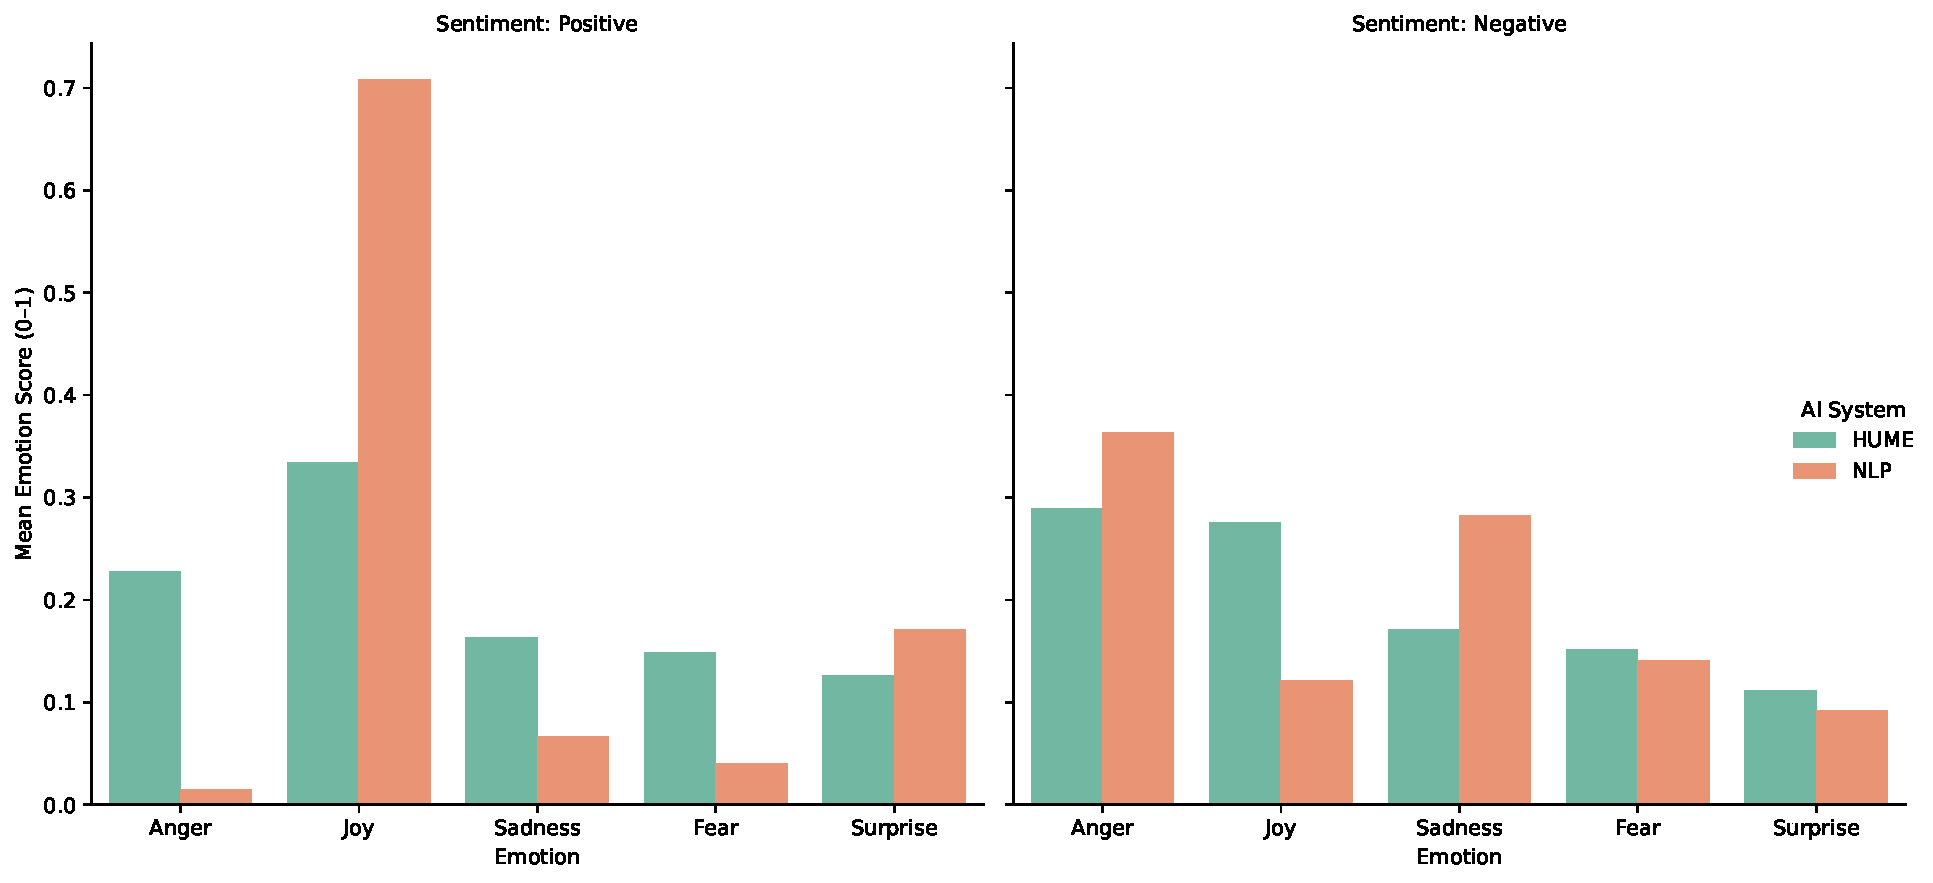
\includegraphics[width=0.95\textwidth]{png/results/rq2/sentiment_comparison_facet_all.pdf}
    \caption{Average emotion score for Hume AI and NLP Cloud, seperated by positive and negative recordnigs.}
    \label{fig:rq2_sent_grouped_bar}
\end{figure}

The differences in the average emotion scoring are presented further in Figure \ref{fig:rq2_avg_diff_full}. Positive values indicate that Hume AI assigned higher scores for respective emotions, while negative values imply higher scores from NLP Cloud. 
As explained for Figure \ref{fig:rq2_sent_grouped_bar}, the most evident difference was shown for joy in both sentiment contexts, where NLP rates it significantly higher in positive settings and Hume higher in negative settings. 
Differences for sadness and surprise were insignificant in negative interviews, aligned with surprise in positive interviews. 
In Figure \ref{fig:rq2_avg_diff_full}, the divergence in rating of fear in negative contexts is obvious where NLP rated the emotion more frequent. 

\begin{figure}[!h]
    \centering 
    \begin{subfigure}[b]{0.49\textwidth}
        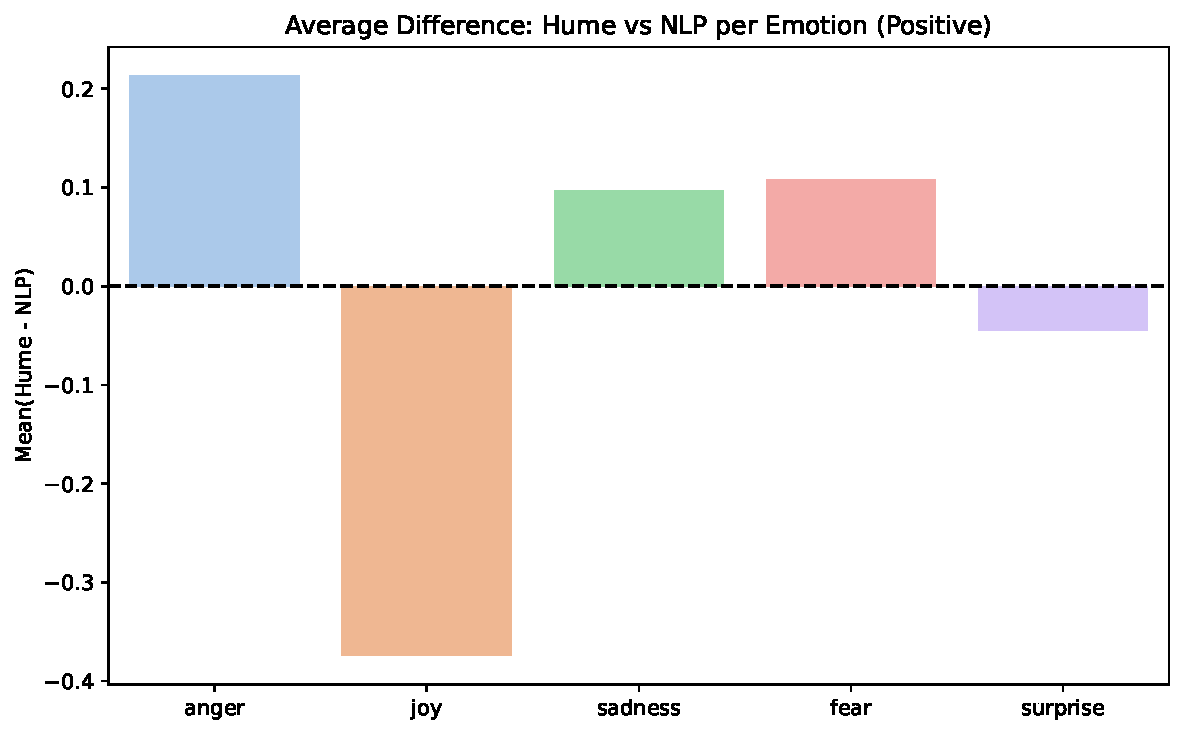
\includegraphics[width=\textwidth]{png/results/rq2/hume_nlp_difference_positive.pdf}
        \caption{Positive recordings.}
        \label{fig:rq2_avg_diff_pos}
    \end{subfigure}
    \begin{subfigure}[b]{0.49\textwidth}
    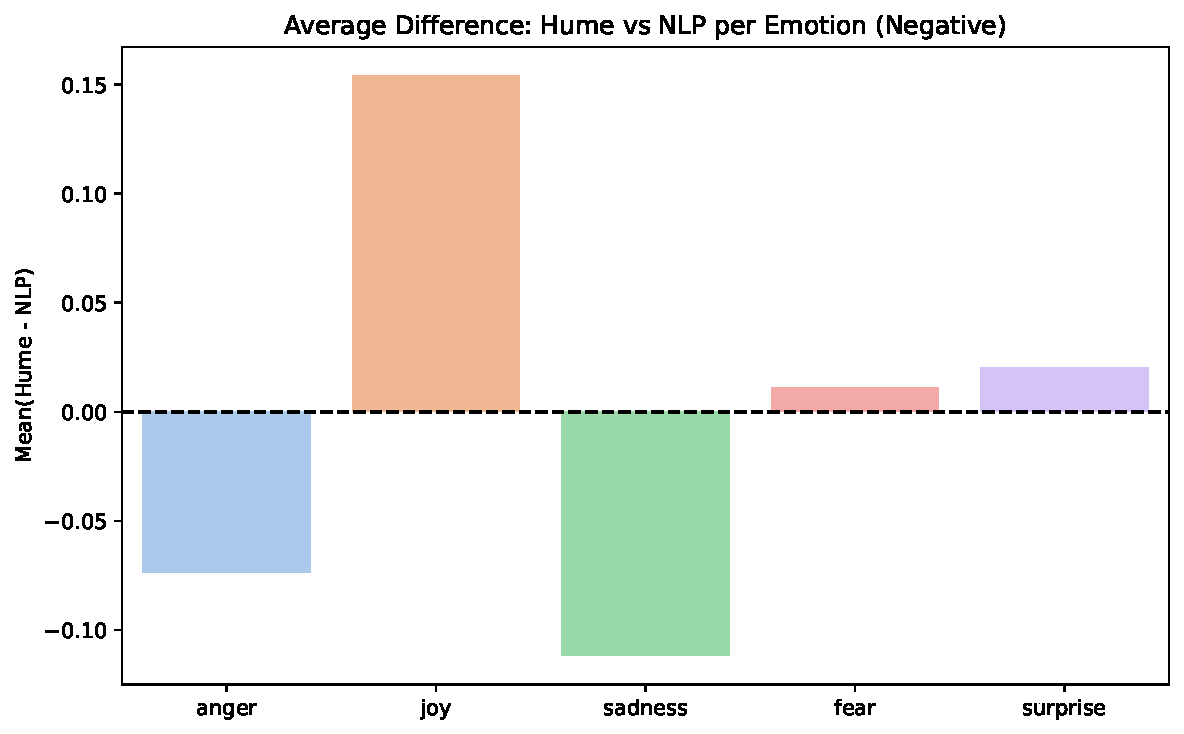
\includegraphics[width=\textwidth]{png/results/rq2/hume_nlp_difference_negative.pdf}
    \caption{Negative recordings.}
    \label{fig:rq2_avg_diff_neg}
    \end{subfigure}
    \caption{Average difference in emotions scores between Hume and NLP.}
    \label{fig:rq2_avg_diff_full}
\end{figure}

\newpage
\subsection{Statistical Analysis}
\subsubsection{Correlation Analysis}

To evaluate how text-based (NLP Cloud) and speech-based (Hume AI) emotion recognition aligns, Pearson correlation coefficients (r) were calculated for each emotion across all interview recordings. 
Table~\ref{tab:corr_all} includes the full dataset (positive and negative recordings), presenting the correlation values as well as corresponding p-values to examine the statistical significance. 

\begin{table}[H]
    \centering
    \caption*{\textbf{All recordings}}
    \begin{tabular}{lrrl}
      \toprule
      \textbf{Emotion} & \textbf{Pearson r} & \textbf{p-value} & \textbf{Significant}\\
      \midrule
      Anger    & 0.466 & 0.007 & Yes \\
      Joy      & 0.521 & 0.002 & Yes \\
      Sadness  & 0.167 & 0.362 & No  \\
      Fear     & 0.171 & 0.348 & No  \\
      Surprise & 0.197 & 0.281 & No  \\
      \bottomrule
    \end{tabular}
    \caption{Pearson Correlations Between NLP and Hume Emotion Scores (Full dataset)}
    \label{tab:corr_all}
  \end{table}

This data demonstrates a reasonable positive correlation for Anger(r = 0.466, p=0.007) and Joy (r=0.521, p=0.0022), implying that these emotions are relatively consistent identified throughout the AI systems on the full dataset. 
The p-values (p<0.05) show a statistical significance and highlights a relevant relationship in how Anger and Joy are detected through different processes. 
Sadness, Fear, and Surprise show contrasted results with weak correlations (r<0.20) where the p-values indicate no significancy with low agreement between the AI models for these emotions when analysing the full dataset. 
Overall, some alignment for the more distinct emotions as Anger and Joy are declared through the correlation analysis, but some difficulties with consistent agreement are prominent for more nuances emotions as Sadness, Fear, and Surprise. 

\begin{table}[H]
    \centering
    \caption*{\textbf{Positive Recordings}}
    \begin{tabular}{lrrl}
      \toprule
      \textbf{Emotion} & \textbf{Pearson r} & \textbf{p-value} & \textbf{Significant}\\
      \midrule
      Anger    & 0.160  & 0.568 & No  \\
      Joy      & 0.682  & 0.005 & Yes \\
      Sadness  & 0.546  & 0.035 & Yes \\
      Fear     & 0.098  & 0.729 & No  \\
      Surprise & -0.050 & 0.860 & No  \\
      \bottomrule
    \end{tabular}
    \caption{Pearson Correlations Between NLP and Hume Emotion Scores (Positive)}
    \label{tab:corr_pos}
  \end{table}
Table \ref{tab:corr_pos} presents the same data as Table \ref{tab:corr_all}, but for positive recordings separately. As for the full dataset, Joy shows a significant correlation (r = 0.682, p = 0.005) between the model’s detection. In contrast, Anger has a lower correlation (r = 0.160, p = 0.568) in positive contexts and Sadness presents a significant correlation (r = 0.549, 0.035) distinct from the full dataset. Fear and Surprise has even lower correlations for positive recordings than the dataset combined, with p-values close to 1. 

\begin{table}[H]
    \centering
    \caption*{\textbf{Negative Recordings}}
    \begin{tabular}{lrrl}
      \toprule
      \textbf{Emotion} & \textbf{Pearson r} & \textbf{p-value} & \textbf{Significant}\\
      \midrule
      Anger    & 0.260 & 0.313 & No  \\
      Joy      & 0.556 & 0.020 & Yes \\
      Sadness  & 0.028 & 0.914 & No  \\
      Fear     & 0.270 & 0.294 & No  \\
      Surprise & 0.209 & 0.422 & No  \\
      \bottomrule
    \end{tabular}
    \caption{Pearson Correlations Between NLP and Hume Emotion Scores (Negative)}
    \label{tab:corr_neg}
  \end{table}
  Table \ref{tab:corr_neg} summerizes the correlation coefficients for the negative recordings. Consistent with the full dataset and positive subset, Joy again demonstrated  a significant correlation in negative contexts (r = 0.556, p = 0.020). 
  All other emotions failed to reach significance, with values that markedly diverged from their corresponding values in the positive recordings: 
  Sadness resulted r = 0.028 (p = 0.914) versus r = 0.546 (p = 0.035) for positives, and Fear showed r = 0.270 (p = 0.294) compared to r = 0.098 (p = 0.729) in the positive context. 



\subsubsection{Paired t-Tests and Effect Sizes}
To further explore alignment and differences between speech-based (Hume AI) and text-based (NLP Cloud) emotion recognition, paired t-tests and Cohen's d were conducted. 
Table \ref{tab:t-test-all} shows the t-statistics, p-values, and Cohen's d for each emotion across the full dataset. Positive t-values implies that Hume rated that emotion more frequent than NLP, negative t-values suggest the opposite.

\begin{table}[H]
    \centering
    \caption*{\textbf{Full Dataset}}
    \begin{tabular}{lrrlr}
      \toprule
      \textbf{Emotion} & \textbf{t‐statistic} & \textbf{p‐value} & \textbf{Significant} & \textbf{Cohen’s d} \\
      \midrule
      Anger    &  1.717 & 0.096  & No  &  0.303 \\
      Joy      & -1.726 & 0.094  & No  & -0.305 \\
      Sadness  & -0.548 & 0.588  & No  & -0.097 \\
      Fear     &  3.341 & 0.002  & Yes &  0.591 \\
      Surprise & -0.657 & 0.516  & No  & -0.116 \\
      \bottomrule
    \end{tabular}
    \caption{t‐statistics, p‐value with significance, and Cohen’s d for all clips.}
    \label{tab:t-test-all}
\end{table}
Across all interviews, only Fear had statistically significant difference between the AI-models (t = 3.341, p = 0.0022), and had a medium effect size (Cohen's d = 0.591).
Hume AI rated fear consistently higher than NLP Cloud, suggesting a systematic modality difference for this emotion. 
Although Anger, Joy, Sadness, and Surprise had some mean-score differences, none reached statistical significance (all p>0.05) and their effect sizes were small (|d| < 0.03). 
Apart from Fear, the two models demonstrated close agreement in recognizing these emotional expressions. 

\begin{table}[H]
    \centering
    \caption*{\textbf{Positive Recordings}}
    \begin{tabular}{lrrlr}
      \toprule
      \textbf{Emotion} & \textbf{t‐statistic} & \textbf{p‐value} & \textbf{Significant} & \textbf{Cohen's d} \\
      \midrule
      Anger    & 10.903  & 0       & Yes & 2.815  \\
      Joy      & -11.665 & 0       & Yes & -3.012 \\
      Sadness  & 6.177   & 0       & Yes & 1.595  \\
      Fear     & 5.125   & 0       & Yes & 1.323  \\
      Surprise & -1.723  & 0.107   & No  & -0.445 \\
      \bottomrule
    \end{tabular}
    \caption{t‐statistics, p‐value with significance, and Cohen's d for positive interviews.}
    \label{tab:t-test-pos}
\end{table}
Table \ref{tab:t-test-pos} demonstrates t-tests and Cohen's d for positive oriented interviews, where all emotions except for surprise (t = -1.723, p = 0.107, d = -0.445) shows significant differences (p < 0.001)
with certainly large effect sizes. Negative T-value and Cohen's d for Joy (t = -11.665, d = -3.012) indicates that NLP have the aspects of overestimating this emotion compared to Hume with large effect sizes, where Hume in contrast tends to overestimate Anger (t = 10.903, d = 2.815) in positive contexts. 
Hume rates Sadness and Fear more prominent than NLP, and Surprise remain inconsistent as previous results with no significant difference (t = -1.723, p = 0.107). 

\begin{table}[H]
    \centering
    \caption*{\textbf{Negative Recordings}}
    \begin{tabular}{lrrlr}
      \toprule
      \textbf{Emotion} & \textbf{t-statistic} & \textbf{p-value} & \textbf{Significant} & \textbf{Cohen’s d} \\
      \midrule
      Anger    & -1.702 & 0.108   & No  & -0.413 \\
      Joy      &  3.720 & 0.002   & Yes &  0.902 \\
      Sadness  & -3.796 & 0.002   & Yes & -0.921 \\
      Fear     &  0.536 & 0.599   & No  &  0.130 \\
      Surprise &  1.311 & 0.208   & No  &  0.318 \\
      \bottomrule
    \end{tabular}
    \caption{t-statistics, p-value with significance, and Cohen’s d for negative interviews.}
    \label{tab:t-test-neg}
  \end{table}
Table \ref{tab:t-test-neg} presents conducted t-tests and Cohen's d in negative interviews, with significant differences for Joy (t = 3.720, p = 0.002), where Hume rates it significantly higher than NLP. 
In contrast, NLP has clear higher scoring for Sadness with large effect size (t = -3.796, d = -0.921). However, the effect sizes are not as big as for the positive recordings. 
For example, the effect sizes for Joy (t = 0.902) are lower than Joy in positive contexts (t = -3.012) where NLP overestimated the emotion compared to Hume.
Anger has a moderate difference, even if it is not statistically significant. No notable differences are detected for either Fear or Surprise. 
This implies that the AI systems strongly disagrees on Joy and Sadness detection in the negative contexts of the dataset. 

\subsubsection{Conclusion Statistical Analysis}
Comparison of speech-based (Hume AI) and text-based (NLP Cloud) with statistical analysis demonstrates correlation particularly for clear expressed emotions as Anger and Joy when analysing the full dataset. 
However, anger shows no correlation between the models for either positive or negative recordings when separated. Joy shows a significant correlation throughout all sentiment contexts, 
where t-tests confirmed that NLP had higher predictions for joy in positive contexts and Hume in negative. 
Emotions that are more subtle like Sadness, Fear, and Surprise, revealed low correlations for all sentiment contexts except positive that showed a strong correlation for sadness, indicating modality-specific distinctions. 
Paired t-tests strengthened this observation regarding the full dataset and negative subset, pointing out Fear as the only emotion with statistically significant divergence in the full dataset where speech-based analysis assigned higher scores consistently. 
However, negative recordings showed significant difference for joy and sadness, while positively oriented clips showed significant difference for all emotions except surprise. 







\subsubsection{Conclusion Sentiment-Based Analysis}
In conclusion, Hume AI and NLP Cloud show moderate to strong agreement on anger (r = 0.47) and joy (r = 0.52) across the full dataset, but weak correlations on sadness, fear, and surprise. Paired t-tests showed that fear is the single emotion that exhibits a significant mean difference across the full interview set (Hume > NLP, d = 0.59), while joy and anger showed modality divergencies in positive and negative subsets where NLP overestimated joy in positive interviews (d = 3.01) and Hume overestimated anger (d = 2.82). These results suggest that text and speech modalities agree on certain emotions particularly when considering the full dataset. However, divergencies occur for sentiment-specific analyses, especially for positive interviews. 

\subsubsection{Case Example}
single clip comparison 

breifly illustrate how speech vs text differ in practice 

\subsection{Conclusion of RQ2 Data Analysis}
The results of this research question show that even if Hume AI and NLP Cloud partially aligns in detecting emotions, certainly for clearly expressed emotions such as Anger and Joy, 
they diverge significantly in their predictions of more nuanced emotions such as Fear, Sadness, and Surprise. Statistical tests confirmed a significant difference for Fear. 
Sentiment-based analysis showed that emotional context have an impact on the results, when analysing five basic emotions, where positive scenarios had a larger model divergence. 
As discussed above, the interview setting and overall data collection may have different impacts on the results. Still, the findings highlights how speech- and text-based models are complementary, each 
with their own strenghts to capture different aspects of emotion expression, and indicate that relying on a single modality could have limitations for comprehensive emotion detection in speech.  


%%%%%%%%%%%%%%%%%%%%%%%%%%%%%%%%%%%%%%%%%%%%%%%%%%%%%%%%%%%%%%%%%%%%%%%%%%%%%%%%%%%%%%%%%%
                        %%%%%%%%%%%%%%%%%%%%% RQ3   %%%%%%%%%%%%%%%
%%%%%%%%%%%%%%%%%%%%%%%%%%%%%%%%%%%%%%%%%%%%%%%%%%%%%%%%%%%%%%%%%%%%%%%%%%%%%%%%%%%%%%%%%%
\section{Data Analysis for RQ3: AI and self-assessed emotion labels}

The third research question explores how AI-generated emotion labels - from both speech-based (Hume AI) and text-based (NLP Cloud) – aligns with participants’ own emotion ratings, to evaluate the agreement and divergence in different interview sentiments (positive and negative). This section includes average emotion scores from self-reports, Hume AI, and NLP Cloud across all recordings and for each sentiment category. Linear agreements are quantified with Pearson correlations and mean-level differences are analysed with paired t-tests and Cohen’s d for assess effect sizes. This approach allows to see the overall alignment between AI-models and participants own assessment as well as how it depends on the sentiment context. 
\subsection{Model Emotion Score and Self-Reports Comparison}

An initial overview is summarised in Table~\ref{tab:rq3_emotion-stats-combined}, Table~\ref{tab:rq3_emotion-stats-pos}, and Table~\ref{tab:rq3_emotion-stats_neg} (\ref{sec:datacoll_rq2_rq3} Data Collection),
with average emotion scores across all 30 interview recordings for each emotion category (anger, joy, sadness, fear, surprise). The table presents mean values and standard deviation for self-resported scores 
aside both AI-systems.Table~\ref{tab:rq3_emotion-stats-pos} includes the same values for positive recordings and Table~\ref{tab:rq3_emotion-stats_neg} presents the data from negative recordings.

These differences are visualized in Figure~\ref{fig:comp-bar-rq3-all}, illustrating a bar chart that compares the average emotion scores defined by 
Hume AI, NLP Cloud, and participants self-assessment seperated by positive and negative oriented interviews.

\begin{figure}[!h]
    \centering
    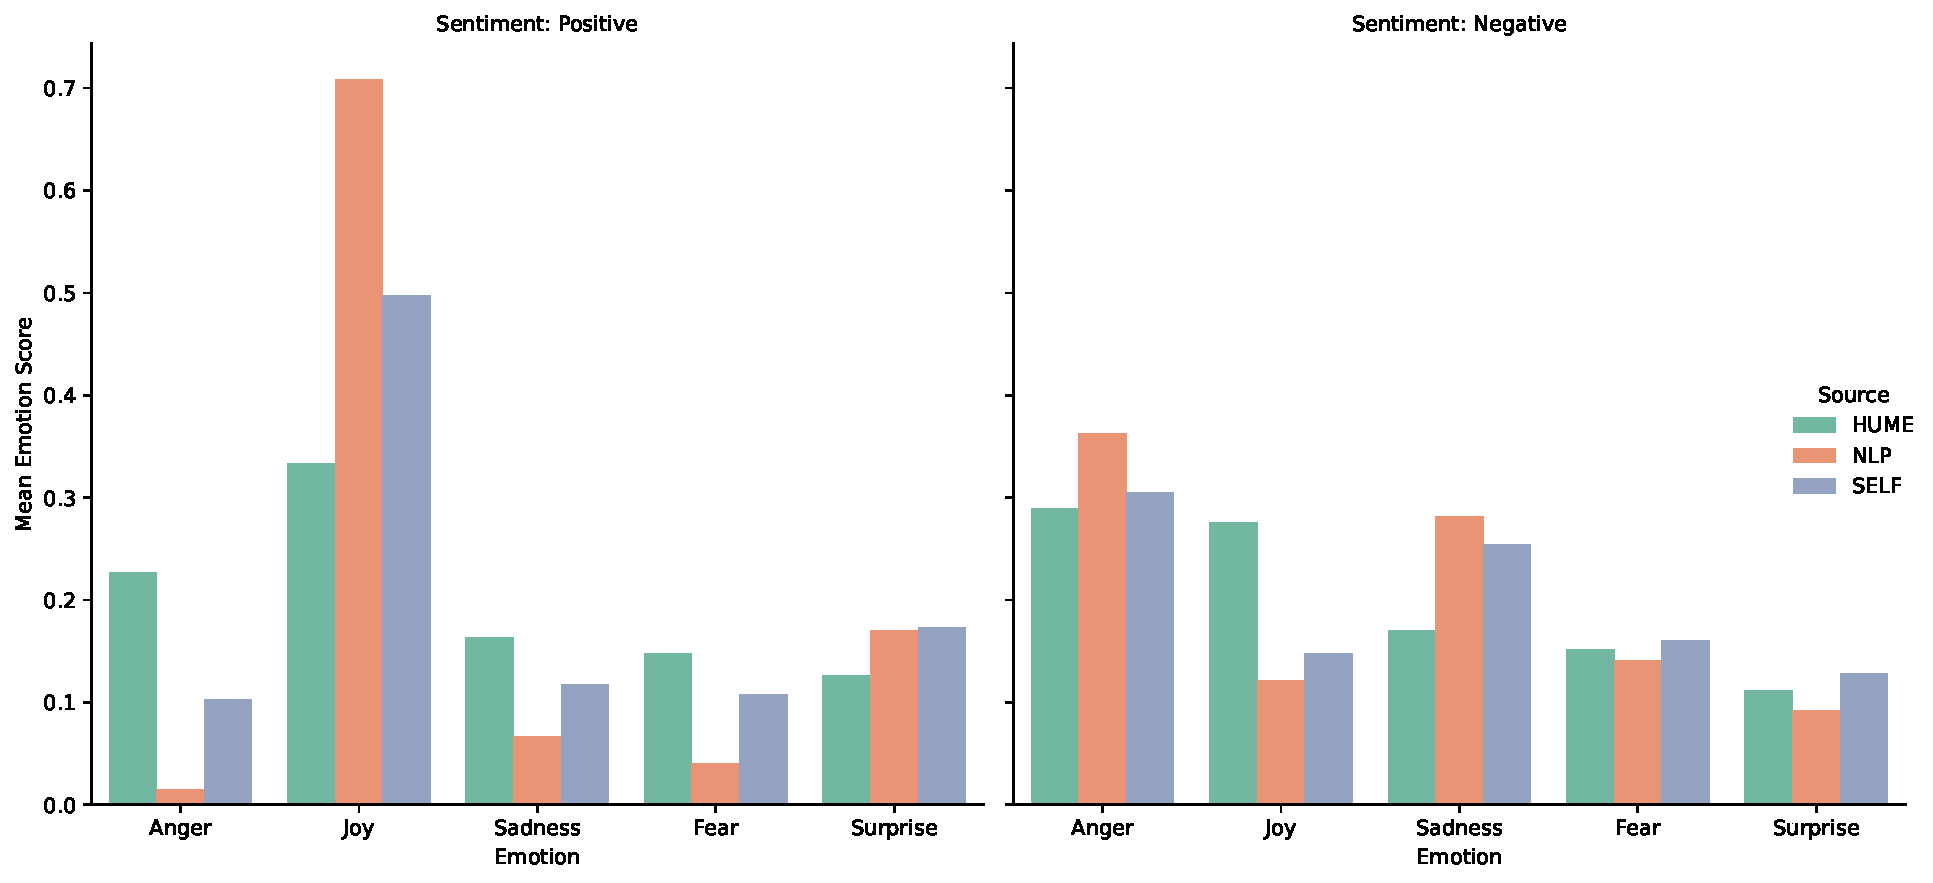
\includegraphics[width=0.95\textwidth]{png/results/rq3/rq3_sentiment_grouped_bar.pdf}
    \caption{Comparison of emotional labels for Hume, NLP, and self-assessed.}
    \label{fig:comp-bar-rq3-all}
\end{figure}

For the positive recordings, Joy consistently had higher self-reported scores than other emotions. NLP rates Joy higher than the participants while Hume rates it lower. 
In contrast, Joy was markedly rated higher by Hume in negative contexts than NLP and self-reporting which rated the emotion equally. The negative related emotions (Anger, Sadness, Fear) were assessed at lower levels by participants in the positive interviews. 
Self-assessed scores generally matched Hume’s higher detection of Sadness, Fear and Surprise than NLP’s minor predictions. Anger had higher rating by Hume than both self-reports and NLP in positive contexts. 
Surprise had similar average score across all sources, slightly lower detection rate by Hume. 

For negative recordings, Anger had similar rating across all sources, with slightly higher rating by NLP.  Joy has markedly higher average score by Hume compared to the other sources, while the speech-model rates Sadness lower than the text-model and participants. 
Fear and surprise had aligned rating by all sources, with a similar pattern where both emotions are rated slightly higher by the participants, closely followed by Hume and lowest rating by NLP. 

This comparison suggests that emotional ranking are more aligned in for the negative recordings, where Joy is the emotion most distinct in the rating by Hume. 
The positive oriented interviews have more varying results between the sources, Joy are significanly rated higher by NLP while the text-based model rates Anger close to zero compared to Hume that rates this emotion higher than all other emotions except for Joy. 

The sentiment-based comparison clearly presents that emotional expression and self-awareness have a signficant variance between modalities and emotional contexts. 
Explicit emotions articulated in words are closely aligned between self-assessed rating and text-based analysis. 
While implicit or suble emotions expressed through vocal tone have a notable divergence. 

\subsection{Correlation and Visual Analysis}
To evaluate the alignment between AI-generated emotion scores and participants self-reported emotions, 
Pearson correlation analyses were conducted across the five emotion categories for both speech-based (Hume AI) and text-based (NLP Cloud) compared to self-reporting.
With these measurements the relationship's strength and direction and the statistical significance can be reviewed. 

\subsubsection{Hume AI vs Self-Reported Emotions}
%%% Correlation hume self 
\begin{table}[H]
    \centering
    \caption*{\textbf{All Hume}}
    \begin{tabular}{lrrl}
      \toprule
      \textbf{Emotion} & \textbf{Pearson’s r} & \textbf{p-value} & \textbf{Significant} \\
      \midrule
      Anger    & 0,359 & 0,043 & Yes \\
      Joy      & 0,334 & 0,062 & No  \\
      Sadness  & 0,050 & 0,784 & No  \\
      Fear     & \(-\)0,007 & 0,969 & No  \\
      Surprise & 0,088 & 0,631 & No  \\
      \bottomrule
    \end{tabular}
    \caption{Pearson’s r, p-values, and significance for all Hume recordings.}
    \label{tab:rq3_corr-hume-all}
  \end{table}

The correlation results for Hume AI predictions on all recordings in the dataset is demonstrated in Table~\ref{tab:rq3_corr-hume-all}, and indicate generally weak correlations across the majority of emotions. 
Anger is the only emotion showing a statistic significant correlation (r = 0.359, p = 0.043), which indicates a moderate alignment between Hume AI's speech based emotion 
detection and participants own perception for this emotion. Joy shows a moderate correlation but without statistical significance (r = 0.334, p = 0.062), other emotions, such as Fear (r = 0.007, p = 0.969), presents no relevant correlation. 

\begin{table}[H]
    \centering
  
    \begin{subtable}{0.45\textwidth}
      \centering
      \caption{\textbf{Positive Recordings (Hume)}}
      \label{tab:rq3_corr-hume-pos}
      \begin{tabular}{l r r r}
        \toprule
        \textbf{Emotion} & \(\mathbf{r}\) & \(\mathbf{p}\) & \textbf{Sign.} \\
        \midrule
        Anger    &  0.404 & 0.136 & No  \\
        Joy      &  0.401 & 0.138 & No  \\
        Sadness  &  0.320 & 0.244 & No  \\
        Fear     & –0.027 & 0.924 & No  \\
        Surprise &  0.091 & 0.748 & No  \\
        \bottomrule
      \end{tabular}
    \end{subtable}\hfill
    \begin{subtable}{0.45\textwidth}
      \centering
      \caption{\textbf{Negative Recordings (Hume)}}\label{tab:rq3_corr-hume-neg}
      \begin{tabular}{l r r r}
        \toprule
        \textbf{Emotion} & \(\mathbf{r}\) & \(\mathbf{p}\) & \textbf{Sign.} \\
        \midrule
        Anger    & –0.105 & 0.690 & No  \\
        Joy      &  0.127 & 0.627 & No  \\
        Sadness  & –0.146 & 0.576 & No  \\
        Fear     & –0.036 & 0.891 & No  \\
        Surprise & –0.143 & 0.585 & No  \\
        \bottomrule
      \end{tabular}
    \end{subtable}
  
    \caption{Pearson’s r, p-values, and significance for Hume AI vs.\ self (positive and negative).}
    \label{tab:rq3_corr-hume-pos-neg}
  \end{table}

Table \ref{tab:rq3_corr-hume-pos} presents correlation coefficients for positive recordings with no significant agreement occurs between Hume predictions and self-reported emotions. Anger, sadness, and sadness show moderate correlations (r = 0.320-0.404) with no statistical significance (p = 0.136-0.244). Weak correlation appears for both fear and surprise with high p-values suggesting no convincing evidence for these correlations. 

Negatively oriented interviews, Table~\ref{tab:rq3_corr-hume-neg} show similar results as for positive interviews where no correlations of significance are found (r = -0.146-0.127, p = 0.576-0.0.891). Four out of five emotion correlations are negative while joy has a weak positive relationship. Each correlation is considered weak without statistical significance, implying that Hume predicted emotions distinct from participants own evaluation.  
%%% Self vs NLP 
\subsubsection{NLP Cloud vs Self-Reported Emotions}
\label{sec:nlp-self}
\begin{table}[H]
    \centering
    \caption*{\textbf{All NLP}}
    \begin{tabular}{lrrr}
      \toprule
      \textbf{Emotion} & \textbf{Pearson’s r} & \textbf{p-value} & \textbf{Significant} \\
      \midrule
      Anger    & 0,739 & 0,000 & Yes \\
      Joy      & 0,863 & 0,000 & Yes \\
      Sadness  & 0,710 & 0,000 & Yes \\
      Fear     & 0,669 & 0,000 & Yes \\
      Surprise & 0,092 & 0,616 & No  \\
      \bottomrule
    \end{tabular}
    \caption{Pearson’s r, p-values, and significance for all NLP recordings.}
    \label{tab:rq3_corr-nlp-all}
  \end{table}

  Table \ref{tab:rq3_corr-nlp-all} presents correlation coefficients between self-reported and NLP-predicted emotions for the full dataset.
  When analysing the full dataset, NLP Cloud demonstrated strong and statistically significant correlations with self-reporting for four of five emotions. Joy showed the strongest correlation (r = 0.863, p < 0.001), followed by Anger (r = 0.739, p < 0.001) and Sadness (r = 0.710, p < 0.001). 
Fear had a moderately strong correlation with high statistical significance (r = 0.669, p < 0.001). Surprise was the single emotion showing weak correlation with no statistical significance (r = 0.092, p = 616). 
  
\begin{table}[H]
    \centering
  
    \begin{subtable}{0.45\textwidth}
      \centering
      \caption{\textbf{Positive Recordings (NLP)}}\label{tab:rq3_corr-nlp-pos}
      \begin{tabular}{l r r r}
        \toprule
        \textbf{Emotion} & \(\mathbf{r}\) & \(\mathbf{p}\) & \textbf{Sign.} \\
        \midrule
        Anger    & –0.199 & 0.477 & No  \\
        Joy      &  0.622 & 0.013 & Yes \\
        Sadness  &  0.363 & 0.183 & No  \\
        Fear     &  0.527 & 0.043 & Yes \\
        Surprise &  0.011 & 0.969 & No  \\
        \bottomrule
      \end{tabular}
    \end{subtable}\hfill
    \begin{subtable}{0.45\textwidth}
      \centering
      \caption{\textbf{Negative Recordings (NLP)}}\label{tab:rq3_corr-nlp-neg}
      \begin{tabular}{l r r r}
        \toprule
        \textbf{Emotion} & \(\mathbf{r}\) & \(\mathbf{p}\) & \textbf{Sign.} \\
        \midrule
        Anger    &  0.286 & 0.266 & No  \\
        Joy      &  0.366 & 0.149 & No  \\
        Sadness  &  0.429 & 0.086 & No  \\
        Fear     &  0.599 & 0.011 & Yes \\
        Surprise & –0.146 & 0.575 & No  \\
        \bottomrule
      \end{tabular}
    \end{subtable}
  
    \caption{Pearson’s r, p-values, and significance for NLP Cloud vs.\ self (positive and negative)}
    \label{tab:rq3_corr-nlp-pos-neg}
  \end{table}
  
  Table \ref{tab:rq3_corr-nlp-pos} presents correlation data between self-reports and NLP Cloud for positive interviews, where lower alignments between self-reports and NLP is found compared to the full dataset. 
  Only correlations for Joy (r = 0.622, p = 0.013) and Fear (r = 0.527, p = 0.043) are statistically significant. Sadness had a moderate correlation without statistical significance, Anger and Surprise presented weak correlations. 
  
  
Correlation coefficients for negative interviews are presented in Table \ref{tab:rq3_corr-nlp-neg}, with similar results as for the positive interviews with weaker correlations compared to the full dataset. The single strong correlation with statistical significance is Fear (r = 0.599, p = 0.011). 
Moderate correlation is found for Joy (r = 0.366 p = 0.149) and Sadness (r = 0.429, p = 0.086), both with no statistical significance. As for the positive recordings, both Anger and Surprise had weak correlations between NLP and self-reporting. 


\subsubsection{Visual Correlation}

Figure \ref{fig:scatter-anger-rq3-pos} illustrates the correlation between self-reported Anger scores and AI-labelled predictions for positive oriented interviews, while Figure~\ref{fig:scatter-anger-rq3-neg} illustrates the correlated data for negative interviews. 
As shown, Hume shows a moderate positive correlation with no statistical significance (r = 0.40, p = 0.136) where the data points have some spreading around the trend line. NLP Cloud shows a weaker correlation with self-reports for anger (r = -0.20, p = 0.477) than Hume in positive recordings, 
as demonstrated in the Figure~\ref{fig:scatter-anger-rq3-pos} for NLP vs Self where data points are spread out vertically in line with the 0.0 axis. 
\begin{figure}[H]
    \centering
    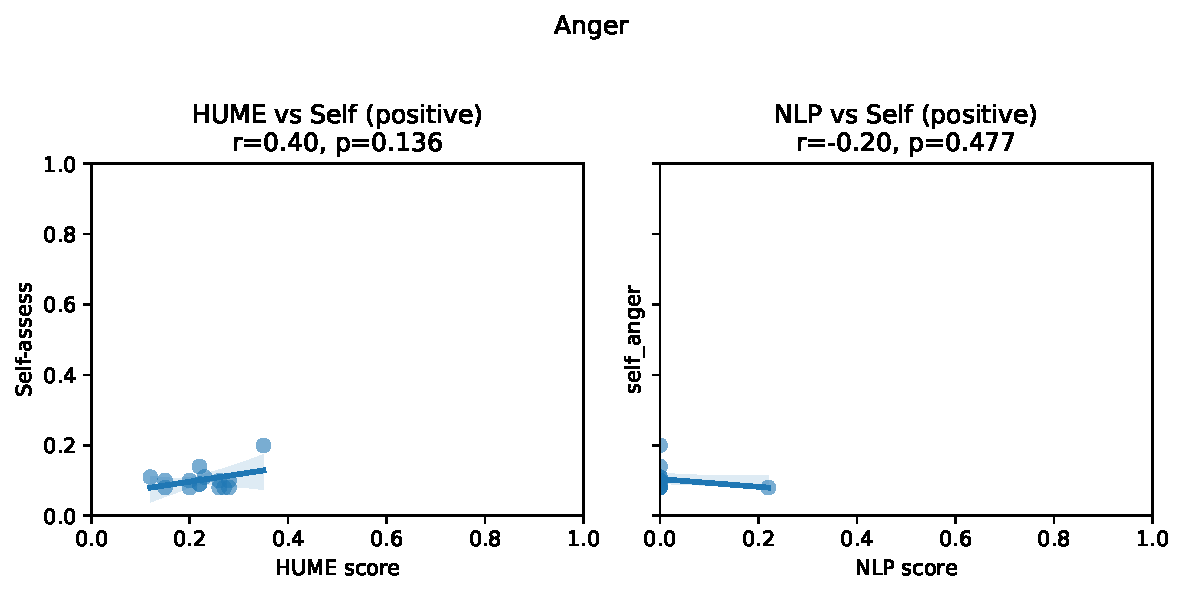
\includegraphics[width=0.7\textwidth]{png/results/rq3/scatter_anger_vs_self_positive.pdf}
    \caption{Scatter plot, Hume, NLP vs. Self for Anger.}
    \label{fig:scatter-anger-rq3-pos}
\end{figure}
The correlation coefficients remain low in Figure~\ref{fig:scatter-anger-rq3-neg}, where NLP presents a moderate positive correlation (r = 0.29, p = 0.266) with self-assessed anger in negative contexts, while the relationship with Hume is weaker (r = -0.10, p = 0.690) than in the positive interviews. The dispersed data points around the trend line visualises the divergence between the AI-systems and participants own judgement. 

\begin{figure}[H]
    \centering
    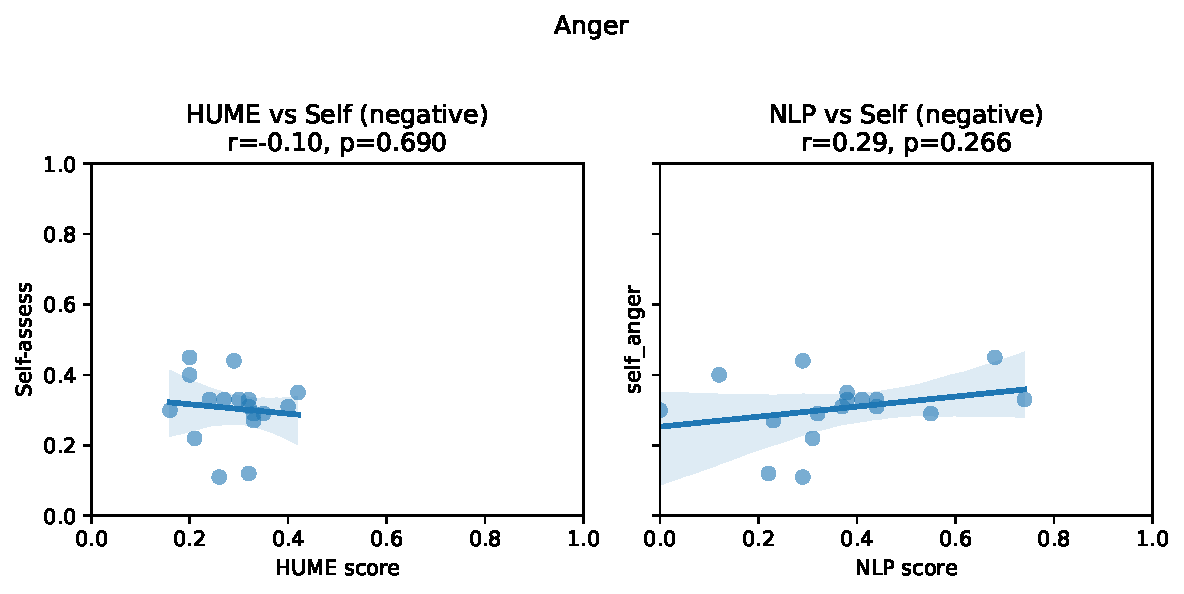
\includegraphics[width=0.7\textwidth]{png/results/rq3/scatter_anger_vs_self_negative.pdf}
    \caption{Scatter plot, Hume, NLP vs. Self for Anger.}
    \label{fig:scatter-anger-rq3-neg}
\end{figure}

Correlations for Joy is presented further in Figure~\ref{fig:scatter-joy-rq3-pos} for positive recordings. Both Hume and NLP show a moderate to strong correlation with self-reported joy, NLP with the strongest correlation with statistical significance (r = 0.62, p = 0.013). This relationship is clearly presented with the data points being relatively close to the trend line for NLP, while the Hume diagram has more dispersed data points. 
\begin{figure}[H]
    \centering
    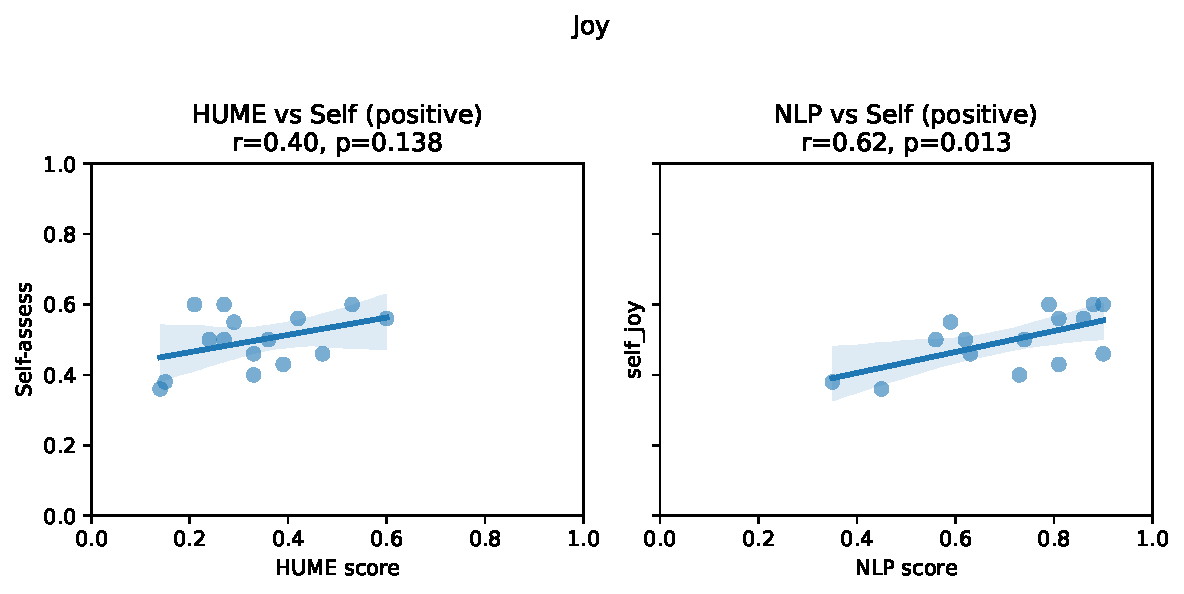
\includegraphics[width=0.7\textwidth]{png/results/rq3/scatter_joy_vs_self_positive.pdf}
    \caption{Scatter plot, Hume, NLP vs. Self for Joy.}
    \label{fig:scatter-joy-rq3-pos}
\end{figure}

Agreement between self-reported and AI-predicted joy is demonstrated for negative interviews in Figure ~\ref{fig:scatter-joy-rq3-neg}.
The trend where NLP has a higher correlation (r = 0.37, p = 0.149) remain, however the moderate relationship has no statistical significance. Hume shows a weak correlation, in contrast with the positive oriented interviews. Data points are more widespread for both Hume and NLP correlation with self-reported joy, suggesting varying rating of this emotion in negative contexts. 
\begin{figure}[H]
    \centering
    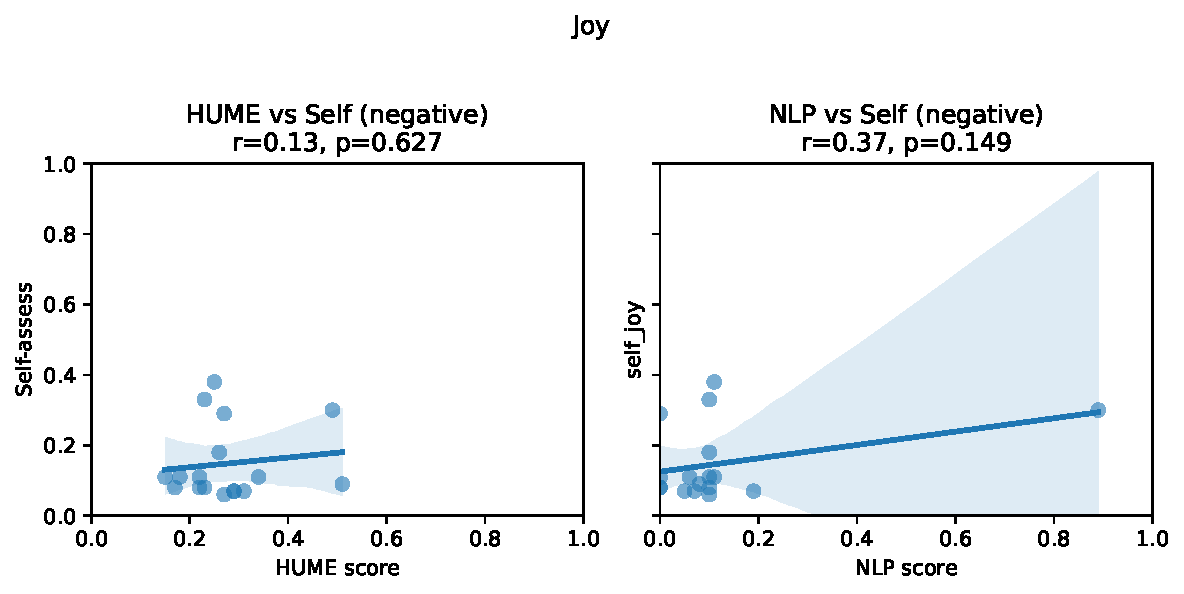
\includegraphics[width=0.7\textwidth]{png/results/rq3/scatter_joy_vs_self_negative.pdf}
    \caption{Scatter plot, Hume, NLP vs. Self for Joy.}
    \label{fig:scatter-joy-rq3-neg}
\end{figure}

\medskip

\subsubsection{Conclusion Correlation and Visual Analysis}

MAYBE INCLUDE TEXT OR DELETE 

\subsection{Statistical Analysis and Effect Sizes}

To explore if AI-generated emotion scores has a significant difference from self-reported emotions, paired t-tests were conducted for both Hume AI and NLP Cloud across each emotion for each sentiment. 
To evaluate the effect size of these differences, Cohen's d were calculated. 

\subsubsection{Hume vs Self-Reports}
Table \ref{tab:rq3_t_hume_self_all} presents the results on paired t-tests with Cohen's d to compare Hume AI's speech-based emotion scores to participants reports across the full dataset. 
As shown, Hume AI ratings on anger are higher than self-reports (t = 2.399, p = 0.023, d = 0.424), suggesting a moderate tendency for Hume overestimating anger compared to participants own perception. 
In contrast, Hume underestimate Surprise relatively to self-reports (t = -2.109, p = 0.043, t = -0.373). No significant differences are found for sadness, fear, and surprise (p > 0.05, |d| < 0.20). 
\begin{table}[H]
    \centering
    \caption*{\textbf{All Recodings}}
    \begin{tabular}{l r r l r}
      \toprule
      \textbf{Emotion} & \textbf{t-statistic} & \textbf{p-value} & \textbf{Significant} & \textbf{Cohen’s d} \\
      \midrule
      Anger    &  2.399 & 0.023 & Yes &  0.424 \\
      Joy      & –0.271 & 0.788 & No  & –0.048 \\
      Sadness  & –1.069 & 0.293 & No  & –0.189 \\
      Fear     &  1.052 & 0.301 & No  &  0.186 \\
      Surprise & –2.109 & 0.043 & Yes & –0.373 \\
      \bottomrule
    \end{tabular}
    \caption{Hume AI vs.\ Self—All Recordings (paired t-test \& Cohen’s d)}
    \label{tab:rq3_t_hume_self_all}
  \end{table}
  
Table \ref{tab:rq3_t_hume_self_side_by_side} seperates these comparisons by sentiment. In positive interviews, four of five emotion comparisons show significant differences. 
Hume tends to remarkably overestimate anger (t = 8.776, p < 0.001, d = 2.266) and underestimate joy (t = -5.112, p < 0.001, d = -1.320), 
and assigning notable higher scores for sadness and fear compared to participants own evaluation. Surprise is the single emotion that remains unsignificant.
In negative interviews, significant differences appears for joy (t = 3.878, p = 0.001, d = 0.941) where Hume predicts higher levels than self-reported scores, and for sadness (t = -2.890, p = 0.013, d = -0.677) that is rated higher by participants than Hume. 
Other emotions show no reliable difference. 

  \begin{table}[H]
    \centering
    \begin{subtable}{0.45\textwidth}
      \centering
      \caption{Positive Recordings}\label{tab:rq3_t_hume_self_pos}
      \begin{tabular}{l r r l r}
        \toprule
        \textbf{Emotion} & \(\;t\;\) & \(\;p\;\) & \textbf{Sign.} & \(\;d\;\) \\
        \midrule
        Anger    &  8.776 & 0.000 & Yes &  2.266 \\
        Joy      & –5.112 & 0.000 & Yes & –1.320 \\
        Sadness  &  2.451 & 0.028 & Yes &  0.633 \\
        Fear     &  2.463 & 0.027 & Yes &  0.636 \\
        Surprise & –1.855 & 0.085 & No  & –0.479 \\
        \bottomrule
      \end{tabular}
    \end{subtable}\hfill
    \begin{subtable}{0.45\textwidth}
      \centering
      \caption{Negative Recordings}\label{tab:rq3_t_hume_self_neg}
      \begin{tabular}{l r r l r}
        \toprule
        \textbf{Emotion} & \(\;t\;\) & \(\;p\;\) & \textbf{Sign.} & \(\;d\;\) \\
        \midrule
        Anger    & –0.517 & 0.612 & No  & –0.125 \\
        Joy      &  3.878 & 0.001 & Yes &  0.941 \\
        Sadness  & –2.790 & 0.013 & Yes & –0.677 \\
        Fear     & –0.454 & 0.656 & No  & –0.110 \\
        Surprise & –1.033 & 0.317 & No  & –0.250 \\
        \bottomrule
      \end{tabular}
    \end{subtable}
  
    \caption{Paired t-test and Cohen’s d for Hume AI vs.\ Self in positive and negative interviews.}
    \label{tab:rq3_t_hume_self_side_by_side}
  \end{table}
  
These results suggests that Hume AI's speech-based assessments only have weak agreements with participant's self-reports, with varying alignment depending on emotion and sentiment context. 
In positive interviews, the model remarkably over- or underestimates anger and joy compared to self-reported emotions, while in negative interviews the only significant differences occur for joy and sadness. 

\subsubsection{NLP Cloud vs Self-Reports}
Paired t-tests with Cohen's d for comparison of NLP Cloud's text-based emotion scores and participants' self-reports for all recordings are presented in Table~\ref{tab:rq3_t_nlp_self_all}. 
Significant differences are found for joy, where NLP rates it higher than self-reports (t = 2.331, p = 0.026, d = 0.412). In contrast, NLP tends to underestimate fear comparing to self-reports (t = -3.496, p = 0.001, d = 0.618). 
Anger, sadness, and surprise show now significant difference (p > 0.05, |d| < 0.20).  
\begin{table}[H]
    \centering
    \caption*{\textbf{All Recodings}}
    \begin{tabular}{l r r l r}
      \toprule
      \textbf{Emotion} & \textbf{t-statistic} & \textbf{p-value} & \textbf{Significant} & \textbf{Cohen’s d} \\
      \midrule
      Anger    & –0.373 & 0.711 & No  & –0.066 \\
      Joy      &  2.331 & 0.026 & Yes &  0.412 \\
      Sadness  & –0.525 & 0.603 & No  & –0.093 \\
      Fear     & –3.496 & 0.001 & Yes & –0.618 \\
      Surprise & –1.011 & 0.320 & No  & –0.179 \\
      \bottomrule
    \end{tabular}
    \caption{Paired t-tests and Cohen's d for NLP Cloud vs.\ Self. All Recordings}
    \label{tab:rq3_t_nlp_self_all}
  \end{table}
  
Table \ref{tab:rq3_t_nlp_self_side_by_side} seperates the comparisons by sentiment. In positive interviews, NLP rates anger at significantly lower levels than participants (t = -4.853, p < 0.001, d = -1.253), while rating 
joy higher than self-reports (t = 6.066, p < 0.001, d = 1.566). Both sadness and fear have a significant difference where NLP tends to underestimate these emotions compared to self-reports. Surprise remains without significance. 
In negative oriented recordings, no significant difference between NLP and self-reports are found (p > 0.05, |d| < 0.389), suggesting closer alignment during negative contexts. 

  \begin{table}[H]
    \centering
  
    \begin{subtable}{0.45\textwidth}
      \centering
      \caption{Positive Recordings}\label{tab:rq3_t_nlp_self_pos}
      \begin{tabular}{l r r l r}
        \toprule
        \textbf{Emotion} & \(\mathbf{t}\) & \(\mathbf{p}\) & \textbf{Sign.} & \(\mathbf{d}\) \\
        \midrule
        Anger    & –4.853 & 0.000 & Yes & –1.253 \\
        Joy      &  6.066 & 0.000 & Yes &  1.566 \\
        Sadness  & –2.852 & 0.013 & Yes & –0.736 \\
        Fear     & –4.603 & 0.000 & Yes & –1.188 \\
        Surprise & –0.075 & 0.941 & No  & –0.019 \\
        \bottomrule
      \end{tabular}
    \end{subtable}\hfill
    \begin{subtable}{0.45\textwidth}
      \centering
      \caption{Negative Recordings}\label{tab:rq3_t_nlp_self_neg}
      \begin{tabular}{l r r l r}
        \toprule
        \textbf{Emotion} & \(\mathbf{t}\) & \(\mathbf{p}\) & \textbf{Sign.} & \(\mathbf{d}\) \\
        \midrule
        Anger    &  1.335 & 0.200 & No  &  0.324 \\
        Joy      & –0.578 & 0.571 & No  & –0.140 \\
        Sadness  &  1.073 & 0.299 & No  &  0.260 \\
        Fear     & –1.149 & 0.267 & No  & –0.279 \\
        Surprise & –1.604 & 0.128 & No  & –0.389 \\
        \bottomrule
      \end{tabular}
    \end{subtable}
  
    \caption{Paired t-test and Cohen’s d for NLP Cloud vs.\ Self in positive and negative interviews.}
    \label{tab:rq3_t_nlp_self_side_by_side}
  \end{table}

Overall, these results implies that NLP Cloud have higher agreement with self-reports in negative contexts, but in positive interviews notable divergencies are found for certain emotions, most appearing for anger, joy and fear.


\subsection{Conclusion of RQ3 Data Analysis}
The result for the full dataset shows that Hume AI only has two small significant divergencies from self-reports, where anger is overestimated (d = 0.42) and surprise underestimated (d = -0.37) compared to ratings by the participants, while all other emotions show no significance in t-tests and weak correlations. When separated by sentiment, Hume tends to overestimate anger and underestimate joy relatively to self-reports in positive contexts, in negative interviews it diverges on joy and sadness. 
In contrast, NLP Cloud are closely aligned with self-reports in negative contexts, with no significant differences, but in positive interviews NLP remarkedly underestimates anger (d = -1.25), rates fear at lower levels, and joy at higher levels compared to self-reports.  compared to self-reports. Correlation analyses strengthen these patterns, where NLP correlations with self-assessed scores are strong for anger, joy, sadness, and fear in the full set, and Hume only shows a moderate correlation for anger and weaker correlations for other emotions. However, the correlations are not as strong when separating the interviews by sentiment. 
Overall, text-based emotion detection with NLP Cloud has higher agreement with participants’ self-assessments, especially in negative interviews, while speech-based detection with Hume have more variations between positive and negative contexts. These results shows that each modality captures distinct features when comparing with human-labelled rating of their own emotions, and the alignment is fluctuating depending on the interview sentiment.  
  